

\newpage 
\appendix 
\section{Further Related Works}\label{sec:more_related_works}




\paragraph{Decoding in autoregressive models with rewards.} 

The decoding strategy, which dictates how sentences are generated from the model, is a critical component of text generation in autoregressive language models \citep{wu2016google,chorowski2016towards,leblond2021machine}.  Recent studies have explored inference-time techniques for optimizing downstream reward functions \citet{dathathri2019plug,yang2021fudge,qin2022cold,mudgal2023controlled,zhao2024probabilistic,han2024value}. While there are similarities between these works and ours, to the best of our knowledge, no prior work has extended such methodologies to diffusion models. Furthermore, our approach leverages characteristics unique to diffusion models that are not present in autoregressive models such as \alg-PM.






\section{Difference Between {\alg} and ``Standard'' SMC-Methods}\label{sec:filter}




 
{ In this section, we compare our algorithm with the SMC-based methods \citep{wu2024practical,trippe2022diffusion,dou2024diffusion,phillips2024particle,cardoso2023monte} for guidance. While they originally aim to solve a conditioning problem, which is different from reward maximization, they algorithms can be converted to reward maximization. First, we will explain this converted algorithm. We then elaborate on the differences between \alg,\,and them in the context of reward maximization. Notably, our SVDD is an instantiation of nested-IS SMC \citep[Algorithm 5]{naesseth2019elements} in the literature on computational statistics, whereas these SMC-based Methods rely on standard sequential Monte Carlo.
} 

\subsection{SMC-Based Methods}

\begin{algorithm}[!ht]
\caption{Guidance with ``Standard'' SMC (for reward maximization)}\label{alg:SMC}
\begin{algorithmic}[1]
     \STATE {\bf Require}: Estimated value functions $\{\hat v_t(x)\}_{t=T}^0$, pre-trained diffusion models $\{p^{\pre}_t\}_{t=T}^0$, hyperparameter $\alpha \in \RR$, Batch size $N$
     \FOR{$t\in [T+1,\cdots, 0]$}
       \STATE \textbf{IS step:}  \label{line:IS} 
       \STATE $$i \in [1,\cdots, N]; x^{[i]}_{t-1} \sim p^{\pre}_{t-1}(\cdot| x^{[i]}_{t}), w^{[i]}_{t-1}:= \frac{\exp(\hat v_{t-1}(x^{[i]}_{t-1})/\alpha )}{\exp(\hat v_t(x^{[i]}_{t})/\alpha )}$$
        \STATE \textbf{Selection step:} select new indices with replacement \label{line:selection}
       \STATE  $\{x^{[i]}_{t-1}\}_{i=1}^N  \leftarrow \{x^{\zeta^{[i]}_{t-1}}_{t-1}\}_{i=1}^N,\quad \{\zeta^{[i]}_{t-1}\}_{i=1}^N \sim \mathrm{Cat}\left ( \left \{\frac{w^{[i]}_{t-1}}{\sum_{j=1}^N w^{[j]}_{t-1} } \right \}_{i=1}^N \right)$
     \ENDFOR
  \STATE {\bf Output}: $x_0$
\end{algorithmic}
\end{algorithm} 


The complete algorithm of TDS in our setting is summarized in \pref{alg:SMC}. Since our notation and their notations are slightly different, we first provide a brief overview. It consists of two steps. Since our algorithm is iterative, at time point $t$, consider we have $N$ samples (particles) $\{x^{[i]}_{t}\}_{i=1}^N$. 


\paragraph{IS step (\pref{line:IS}).} We generate a set of samples $\{x^{ [i] }_{t-1}\}_{i=1}^N$ following a policy from a pre-trained model  $p^{\pre}_{t-1}(\cdot|\cdot)$. In other words, 
\begin{align*}
 \forall i \in [1,\cdots,N];  x^{[i]}_{t-1} \sim p^{\pre}_{t-1}(\cdot|x^{[i]}_{t}). 
\end{align*} 
Now, we denote the importance weight for the next particle $x_{t-1}$ given the current particle $x_{t}$ as $w(x_{t-1}, x_{t})$, expressed as
\begin{align*}
    w(x_{t-1},x_{t}):=\frac{\exp(v_{t-1}(x_{t-1})/\alpha ) }{\int \exp(v_{t-1}(x_{t-1})/\alpha)p^{\pre}_{t-1}(x_{t-1}|x_{t}) dx_{t-1} }=\frac{\exp(v_{t-1}(x_{t-1})/\alpha) }{ \exp(v_{t}(x_{t})/\alpha) },  
\end{align*}
and define $$\forall i \in [1,\cdots,N];\quad  w^{[i]}_{t-1}:=w(x^{[i]}_{t-1},x^{[i]}_{t}). $$
Note here we have used the soft Bellman equation:
\begin{align*}
        \exp(v_t(x_t)/\alpha )=\int \exp(v_{t-1}(x_{t-1})/\alpha )p^{\pre}_{t-1}(x_{t-1}|x_{t}) dx_{t-1}. 
\end{align*}


Hence, by denoting the target marginal distribution at $t-1$, we have the following approximation: 
\begin{align*}
     p^{\tar}_{t-1}  \underbrace{\approx}_{\text{IS}} \sum_{i=1}^N  \frac{w^{[i]}_{t-1}}{\sum_{j=1}^N w^{[j]}_{t-1} } \delta_{x^{[i]}_{t-1} }. 
\end{align*}

\paragraph{Selection step (\pref{line:selection}).}
Finally, we consider a resampling step. The resampling indices are determined by the following: 
\begin{align*}
    \{\zeta^{[i]}_{t-1}\}_{i=1}^N \sim \mathrm{Cat}\left ( \left \{\frac{w^{[i]}_{t-1}}{\sum_{j=1}^N w^{[j]}_{t-1} } \right \}_{i=1}^N \right). 
\end{align*}
To summarize, we conduct 
\begin{align*}
      p^{\tar}_{t-1}  \underbrace{\approx}_{\text{IS}} \sum_{i=1}^N  \frac{w^{[i]}_{t-1}}{\sum_{j=1}^N w^{[j]}_{t-1} } \delta_{x^{[i]}_{t-1}} \underbrace{\approx}_{\text{Resampling}} \frac{1}{N} \sum_{i=1}^N \delta_{x^{\zeta_{t-1}^{[i]}}_{t-1} }. 
\end{align*}


{Finally, we give several important remarks. 
\begin{itemize}
\item In SMC, resampling is performed across the \emph{entire} batch. However, in the algorithm, sampling is done within a single batch. Therefore, the algorithms differ significantly. We will discuss the implications in the next section.
\item All of existing works \citet{wu2024practical,cardoso2023monte,phillips2024particle,dou2024diffusion} actually consider a scenario where the reward $r$ is a classifier. In \pref{alg:SMC}, we tailor the algorithm for reward maximization. Vice verisa, as we mentioned in \pref{sec:extension}, our \alg\,can also operate effectively when $r$ is a classifier.
\item In \citet{wu2024practical,cardoso2023monte,phillips2024particle}, the proposal distribution is not limited to the pre-trained model. Likewise, in our \alg, we can select an arbitrary proposal distribution, as discussed in \pref{sec:arbitary}. 
    \item In the context of autoregressive (language) models, \citet{zhao2024probabilistic,lew2023sequential} proposed a similar algorithm.  
\end{itemize}
} 

{ \subsection{Comparison of SVDD with ``Standard'' SMC-Based Methods (SSM) for Reward Maximization}
\label{sec:dif_smc_svdd}

We now compare our \alg\,with ``standard'' SMC-Based Methods (SSM). Here, we write a batch size of SVDD in $G$. Importantly, we note that our implementation is analogous to nested-IS SMC in the literature in computational statistics; hence, many differences between nested-IS SMC \citep{naesseth2019elements,naesseth2015nested} and pure SMC in computational statistics are translated here.    


We first reconsider the fundamental assumptions of each algorithm. SVDD's performance, in terms of rewards, depends on the size of $M$ but is independent of the batch size $G$. In contrast, the performance of SSM depends on the batch size $N$. With this in mind, we compare the advantages of SVDD over SSM from various perspectives.

\paragraph{Tailored to optimization in SVDD.} \alg is considered more suitable for optimization than SMC. This is because, when using SMC for reward maximization, we must set $\alpha$ very low, leading to a lack of diversity. This is expected, as when $\alpha$ approaches 0, the effective sample size reduces to 1. This effect is also evident in our image experiments, as shown in \pref{fig:dif_SMC_SVDD}. Although SMC performs well in terms of reward functions, there is a significant loss of diversity. Some readers might think this could be mitigated by calculating the effective sample size based on weights (i.e., value functions) and resampling when the effective size decreases; however, this is not the case, as the effective sample size does not directly translate into greater diversity in the generated samples. In contrast, \alg, maintains much higher diversity.

\begin{figure}[!t]
    \centering
       \begin{subfigure}[b]{0.48\textwidth}
    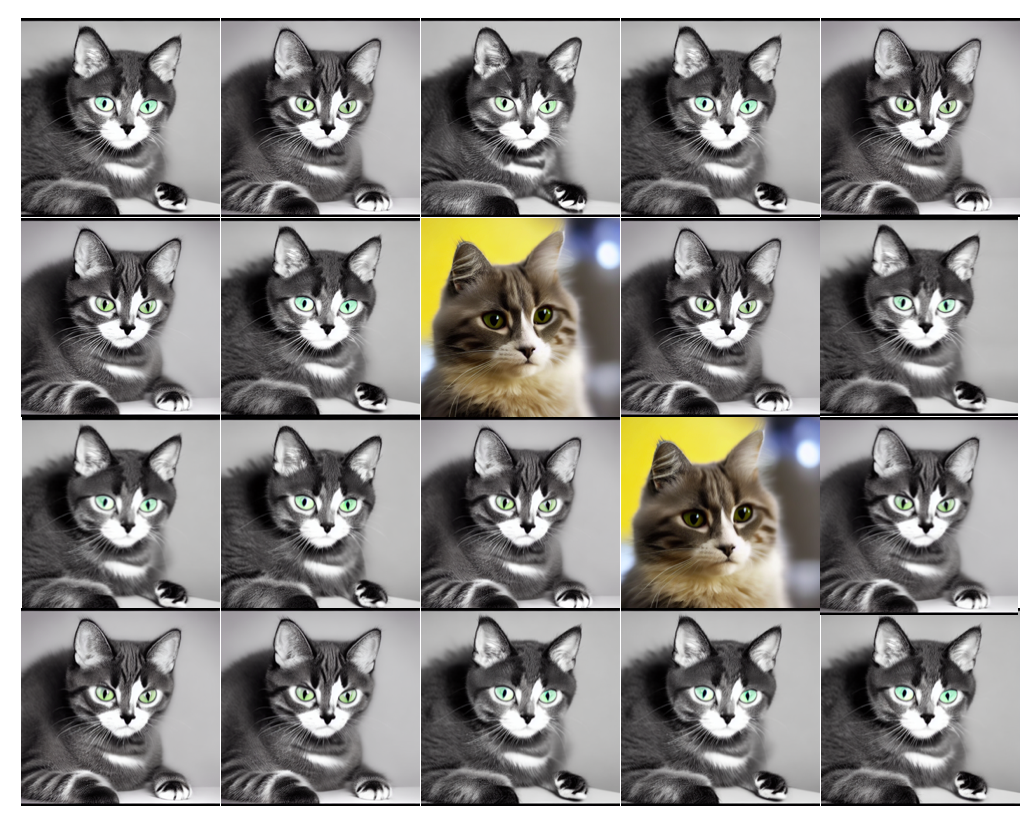
\includegraphics[width=1.0\linewidth]{images/SMC_result.png}
          \caption{Samples from SMC}
       \end{subfigure}%
        \begin{subfigure}[b]{0.48\textwidth} 
    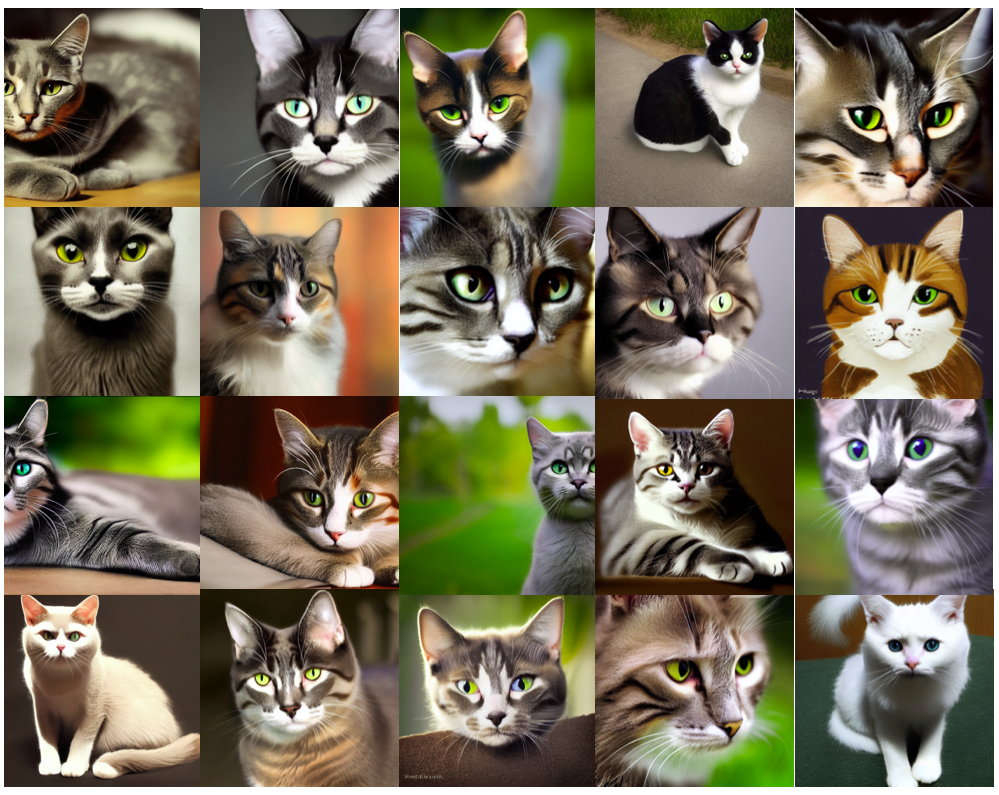
\includegraphics[width=1.0 \linewidth]{images/PM_result.png}
          \caption{Samples from \alg-PM}
       \end{subfigure}
        \begin{subfigure}[b]{0.48\textwidth} 
     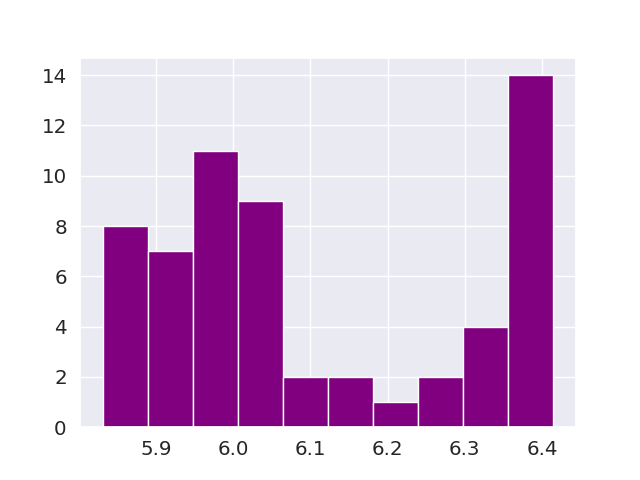
\includegraphics[width= 0.7 \linewidth]{images/SMC_hist.png}
          \caption{Aesthetic scores from SMC}
       \end{subfigure}
         \begin{subfigure}[b]{0.48\textwidth} 
     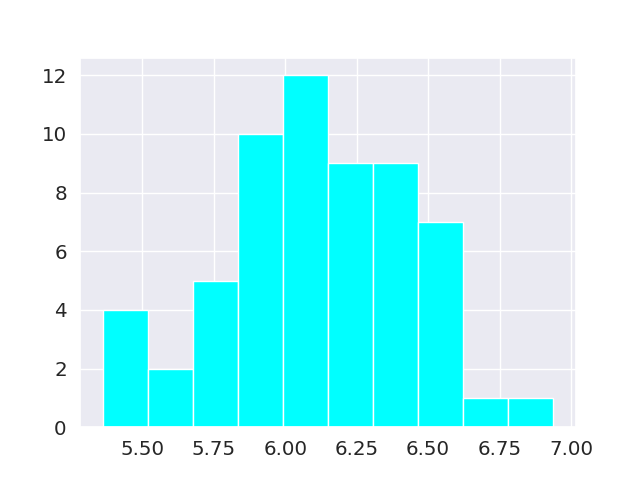
\includegraphics[width=0.7\linewidth]{images/PM_hist.png}
          \caption{Aesthetic scores from \alg-PM}
       \end{subfigure}
       
    \caption{Examples of generated samples from SMC (left) and \alg\,(right), when the prompt is ``cat.'' The histogram of generated samples in terms of the reward function is shown below. Here, the pre-trained models are based on stable diffusion, and we optimize for aesthetic scores. In SMC, we set the batch size $N=60$, and in \alg, we set the duplication size $M=20$. It is observed that most samples generated by SMC are similar, although diversity in terms of reward functions is roughly maintained. This suggests that the effective sample size in terms of value functions (i.e., weights) does not directly translate to real diversity in the generated samples. On the other hand, in SVDD, the generated samples are much more diverse while still achieving high reward functions.    
    }
    \label{fig:dif_SMC_SVDD}
\end{figure}
\paragraph{Ease of parallelization in SVDD.}

SVDD is significantly easier to parallelize across multiple nodes. In contrast, SSM requires interaction between nodes for parallelization. This advantage is also well-documented in the context of nested-IS SMC versus standard SMC \citep{naesseth2019elements}.

\paragraph{High performance of SVDD under memory constraints.}

Now, consider a scenario where the batch size is small, which often occurs due to memory constraints in large pre-trained diffusion models. In this case, while SSM may exhibit suboptimal performance, SVDD-PM can still achieve high performance by choosing a sufficiently large $M$. 


\paragraph{In SSM, the ``ratio'' is approximated.}

In SVDD, we approximate each 
$\exp(v_{t-1}(x_{t-1})/\alpha)$
as a weight. However, in standard SMC, the ratio is approximated as a weight: 
\begin{align*}
 \frac{\exp(v_{t-1}(x_{t-1})/\alpha) }{\exp(v_{t}(x_{t})/\alpha)}.
\end{align*}
The key difference is that in SSM, both the numerator and the denominator are approximated, which could lead to greater error propagation.

} 

{
\section{Comparison against DG \citep{nisonoff2024unlocking} and DiGress \citep{vignac2022digress} in Discrete Diffusion Models}
\label{sec:DG}

Our method is closely related to guidance methods used in DG \citep{nisonoff2024unlocking} and DiGress \citep{vignac2022digress}. However, we emphasize that our approach is more general, as it operates on any domain, including continuous spaces including Riemannian spaces and discrete spaces, in a unified manner. In this sense,  a strict comparison is not feasible. With this in mind, we provide a comparison focusing on cases where all domains are discrete.

\paragraph{Comparison with \citet{nisonoff2024unlocking}.}

In this continuous framework, following the notation in \citep{lou2023discrete}, they propose the use of the following rate matrix: 
\begin{align*} 
Q^{\star}_{x,y}(t) = Q^{\pre}_{x,y}(t)\frac{\exp(v_{t}(y)/\alpha)}{\exp(v_{t}(x)/\alpha)}. 
\end{align*} 
where $Q^{\pre}_{x,y}(t)$ is a rate matrix in the pre-trained model. This suggests that, with standard discretization, the optimal policy at each time step is: 
\begin{align}\label{eq:formula} 
 p(x_{t+\delta t}=y|x_t=x) = \mathrm{I}(x\neq y) + Q^{\star}_{x,y}(t)(\delta t)
\end{align}
where $\delta t$ is step size. Asymptotically, this is equivalent to sampling from the optimal policy in \pref{thm:key}, as we will show in \pref{rem:equivalence}. However, as \citet{nisonoff2024unlocking} note, sampling from the optimal policy requires $O(KL)$ computation, where $K$ is the vocabulary size and $L$ is the sequence length, which is computationally expensive for large $K$ and $L$. To address this issue, they propose using a Taylor approximation by computing the gradient once. However, this is a heuristic in the sense that there is no theoretical guarantee for this approximation. In contrast, we avoid this computational overhead in a different manner, i.e., through importance sampling and resampling. Our algorithm has an asymptotic guarantee as $M$ goes to infinity. Empirically, we have compared two methods in \pref{sec:experiment}. 

\begin{remark}[Asymptotic equivalence between formula in \citet{nisonoff2024unlocking} and \pref{thm:key} ] \label{rem:equivalence}
The informal reasoning is as follows. Recall that the pre-trained policy can be written as
\begin{align*}
  p(x_{t+\delta t}=y|x_t=x) = \mathrm{I}(x\neq y) +  Q^{\pre}_{x,y}(t)(\delta t).  
\end{align*}
Then, \pref{thm:key} states that the optimal policy is 
\begin{align*}
 \frac{ \{ \mathrm{I}(x\neq y) + Q^{\pre}_{x,y}(t)(\delta t)\} \exp(v_{t}(y)/\alpha) }{ \sum_z \{ \mathrm{I}(x\neq z) + Q^{\pre}_{x,z}(t)(\delta t)\} \exp(v_{t}(z)/\alpha)  }. 
\end{align*}
Now, we have 
\begin{align*}
 & \frac{ \{ \mathrm{I}(x\neq y) + Q^{\pre}_{x,y}(t)(\delta t)\} \exp(v_{t}(y)/\alpha) }{ \sum_z \{ I(x\neq z) + Q^{\pre}_{x,z}(t)(\delta t)\} \exp(v_{t}(z)/\alpha)  } \\ 
 &= \frac{\mathrm{I}(x\neq y) + Q^{\pre}_{x,y}(t)(\delta t)\} \exp(v_{t}(y)/\alpha)}{\exp(v_{t}(x)/\alpha) }\times \left\{1+O(\delta t)  \right \} \\
 &\approx \frac{ \{ \mathrm{I}(x\neq y) + Q^{\pre}_{x,y}(t)(\delta t)\} \exp(v_{t}(y)/\alpha)}{\exp(v_{t}(x)/\alpha) }=  \mathrm{I}(x\neq y) +  \frac{  Q^{\pre}_{x,y}(t)(\delta t) \exp(v_{t}(y)/\alpha)}{\exp(v_{t}(x)/\alpha) }. 
\end{align*}
Thus, this recovers the formula \pref{eq:formula}. 
\end{remark}

\paragraph{Comparison with DiGress in \citet{vignac2022digress}.}


\citet{vignac2022digress} proposed a diffusion model for graphs where each sampling and denoising step operates directly on the discrete structure, avoiding continuous relaxation. They discuss how to implement guidance by treating rewards as a classifier. To bypass the exponential computational cost of sampling from the optimal policy ($p^{(\alpha)}$ in \pref{thm:key}), they employ a Taylor expansion. While it requires the calculation of gradients for value functions, then it mitigates the exponential blow-up in computational time. In contrast, we avoid this computational blow-up through importance sampling (IS) and resampling. A detailed empirical comparison between our method and theirs is left for future work.

\begin{remark}
Note that in our molecule generation experiment in \pref{sec:experiment}, we use GDSS \citep{jo2022score}, which operates in continuous space and differs from DiGress.
\end{remark}
} 


{ \section{Extension with Arbitrary Proposal Distribution}\label{sec:arbitary}


Here, we describe the algorithm where the proposal distribution is not necessarily derived from the policy of the pre-trained model, as summarized in \pref{alg:decoding2}. Essentially, we only adjust the importance weight. In practice, we can use the gradient of a differentiable proxy model, such as DPS, as the proposal distribution $q_{t-1}$. Even if the differentiable proxy (value function) models are not highly accurate, our method will still perform effectively since other value function models $\hat v_{t-1}$ can be non-differentiable.

} 

\begin{algorithm}[!th]
\caption{\alg\,(\textbf{S}oft \textbf{V}alue-Based \textbf{D}ecoding in \textbf{D}iffusion Models)}\label{alg:decoding2}
\begin{algorithmic}[1]
     \STATE {\bf Require}: Estimated soft value function $\{\hat v_t\}_{t=T}^0$ (refer to \pref{alg:MC} or \pref{alg:PM}), pre-trained diffusion models $\{p^{\pre}_t\}_{t=T}^0$, hyperparameter $\alpha \in \mathbb{R}$, proposal distribution $\{q_t\}_{t=T}^0$
     \FOR{$t \in [T+1,\cdots,1]$}
       \STATE  Get $M$ samples from pre-trained polices $\{x^{\langle m \rangle}_{t-1}\}_{m=1}^{M} \sim q_{t-1}(\cdot| x_{t}) $, and for each $m$, and calculate  $$ w^{\langle m \rangle}_{t-1}:= \exp(\hat v_{t-1}(x^{\langle m \rangle}_{t-1})/\alpha)\times \frac{p^{\pre}_{t-1}(x^{\langle m \rangle}_{t-1}| x_{t}) }{q_{t-1}(x^{\langle m \rangle}_{t-1}| x_{t})}.$$ \label{line:select2}
        \STATE $ x_{t-1}   \leftarrow  x^{\langle \zeta_{t-1} \rangle }_{t-1} $ after selecting an index: $ \zeta_{t-1}  \sim \mathrm{Cat}\left ( \left \{\frac{w^{\langle m \rangle}_{t-1}}{\sum_{j=1}^{M} w^{\langle j \rangle}_{t-1} } \right \}_{m=1}^{M} \right),\,$ \label{line:select}
     \ENDFOR
  \STATE {\bf Output}: $x_0$
\end{algorithmic}
\end{algorithm}



\section{Soft Q-learning}\label{sec:soft-q}

In this section, we explain soft value iteration to estimate soft value functions, which serves as an alternative to Monte Carlo regression.

\paragraph{Soft Bellman equation.} Here, we use the soft Bellman equation: 
\begin{align*}
    \exp(v_t(x_t)/\alpha )=\int \exp(v_{t-1}(x_{t-1})/\alpha)p^{\pre}_{t-1}(x_{t-1}|x_{t}) dx_{t-1}, 
\end{align*}
as proved in Section 4.1 in \citep{uehara2024understanding}. In other words,
\begin{align*}
 v_{t}(x_{t}) = \alpha \log \{ \EE_{x_{t-1}\sim p^{\pre}(\cdot|x_t) }\left [ \exp(v_{t-1}(x_{t-1})/\alpha) |x_t   \right ]\}. 
\end{align*}

\paragraph{Algorithm.} Based on the above, we can estimate soft value functions recursively by regressing $v_{t-1}(x_{t-1})$ onto $x_t$. This approach is often referred to as soft Q-learning in the reinforcement learning literature \citep{haarnoja2017reinforcement,levine2018reinforcement}. 

\begin{algorithm}[!ht]
\caption{Value Function Estimation Using Soft Q-learning}\label{alg:MC2}
\begin{algorithmic}[1]
     \STATE {\bf Require}:  Pre-trained diffusion models $\{p^{\pre}_t\}^0_{t=T}$, value function model $v(x;\theta)$
    \STATE Collect datasets $\{x^{(s)}_{T},\cdots,x^{(s)}_0\}_{s=1}^S$ by rolling-out $\{ p^{\pre}_t\}_{t=T}^0$ from $t=T$ to $t=0$. 
      \FOR{$j \in [0,\cdots, J] $}
    \STATE  Update $\theta$ by running regression: 
    \begin{align*}
          \theta'_j \leftarrow \argmin_{\theta}\sum_{t=0}^{T} \sum_{s=1}^S \left \{v (x^{(s)}_t;\theta) - v(x^{(s)}_{t-1};\theta'_{j-1}) \right \}^2.
    \end{align*}
     \ENDFOR  
      \STATE {\bf Output}:  $v(x;\theta'_J)$ 
\end{algorithmic}
\end{algorithm}

In our context, due to the concern of scaling of $\alpha$, as we have done in \pref{alg:MC}, we had better use   
\begin{align*}
    v_{t}(x_{t}) = \EE_{x_{t-1}\sim p^{\pre}(\cdot|x_t) }\left [  v_{t-1}(x_{t-1}) |x_t   \right ]. 
\end{align*}
With the above recursive equation, we can estimate soft value functions as in \pref{alg:MC2}. 






\section{Additional Experimental Details}\label{sec:additional} 

We further add additional experimental details. 

\subsection{Additional Setups for Experiments}

\subsubsection{Settings}

\paragraph{Images.} We define compressibility score as the negative file size
in kilobytes (kb) of the image after JPEG compression following \citep{black2023training}. 
We define aesthetic scorer implemented as a linear MLP on top of the CLIP embeddings, which is trained on more than 400k human evaluations. As pre-trained models, we use Stable Diffusion, which is a common text-to-image diffusion model. As prompts to condition, we use animal prompts following \citep{black2023training} such as [Dog, Cat, Panda, Rabbit, Horse,...]. 

\paragraph{Molecules.}

We calculate QED and SA scores using the RDKit~\citep{landrum2016rdkit} library. We use the docking program QuickVina 2~\citep{alhossary2015fast} to compute the docking scores following~\citet{yang2021hit}, with exhaustiveness as 1. Note that the docking scores are initially negative values, while we reverse it to be positive and then clip the values to be above 0, \textit{i.e.}. We compute DS regarding four proteins, {parp1} (Poly [ADP-ribose] polymerase-1),
{5ht1b} (5-hydroxytryptamine receptor 1B), {braf} (Serine/threonine-protein kinase B-raf), and {jak2} (Tyrosine-protein kinase JAK2), which are target proteins that have the highest AUROC scores of protein-ligand binding affinities for DUD-E ligands approximated with AutoDock Vina.


\paragraph{DNA, RNA sequences.}  We examine two publicly available large datasets: enhancers ($n \approx 700k$) \citep{gosai2023machine} and UTRs ($n \approx 300k$) \citep{sample2019human}, with activity levels measured by massively parallel reporter assays (MPRA) \citep{inoue2019identification}. These datasets have been widely used for sequence optimization in DNA and RNA engineering, particularly in advancing cell and RNA therapies \citep{castillo2021machine,lal2024reglm,ferreira2024dna,uehara2024bridging}. In the Enhancers dataset, each $x$ is a DNA sequence of length 200, while $y \in \RR$ is the measured activity in the Hep cell line. In the 5'UTRs dataset, $x$ is a 5'UTR RNA sequence of length 50, and $y \in \RR$ is the mean ribosomal load (MRL) measured by polysome profiling.


\subsubsection{Baselines and Proposals}

We will explain in more detail how to implement baselines and our proposal. We use A100 GPUs for all the tasks. 

\paragraph{SVDD-MC.} In SVDD-MC, we require value function models. For images, we use standard CNNs for this purpose, with the same architecture as the reward model. For molecular tasks, we use a Graph Isomorphism Network (GIN) model \citep{xu2018powerful} as the value function model. Notably, this model is not differentiable w.r.t. inputs. For GIN, we use mean global pooling and the RELU activation function, and the dimension of the hidden layer is 300. The number of convolutional layers in the GIN model is selected from the set \{3, 5\}; and we select the maximum number of iterations from \{300, 500, 1000\}, the initial learning rate from \{1e-3, 3e-3, 5e-3, 1e-4\}, and the batch size from \{32, 64, 128\}.
For the Enhancer task, we use the Enformer model \citep{avsec2021effective} as the value function model. The Enformer trunk has 7 convolutional layers, each having 1536 channels. as well as 11 transformer layers, with 8 attention heads and a key length of 64. Dropout regularization is applied across the attention mechanism, with an attention dropout rate of 0.05, positional dropout of 0.01, and feedforward dropout of 0.4. The convolutional head for final prediction has 2*1536 input channels and uses average pooling, without an activation function. The model is trained using a batch size selected from \{32, 64, 128, 256\}, the learning rate from \{1e-4, 5e-4, 1e-3\}, and the maximum number of iterations from \{5k, 10k, 20k\}.
For the 5'UTR task, we adopt the \href{https://github.com/jacobkimmel/pytorch_convgru?tab=readme-ov-filea}{ConvGRU} model \citep{dey2017gate}. The ConvGRU trunk has a stem input with 4 channels and a convolutional stem that outputs 64 channels using a kernel size of 15. The model contains 6 convolutional layers, each initialized with 64 channels and a kernel size of 5. The convolutional layers use ReLU as the activation function, and a residual connection is applied across layers. Batch normalization is applied to both the convolutional and GRU layers. A single GRU layer with dropout of 0.1 is added after the convolutional layers. The convolutional head for final prediction uses 64 input channels and average pooling, without batch normalization. For training, the batch size is selected from \{16, 32, 64, 128\}, the learning rate from \{1e-4, 2e-4, 5e-4\}, and the maximum number of iterations from \{2k, 5k, 10k\}.
All function models are trained to converge in the learning process using MSE loss.

\paragraph{SVDD-PM.} For this proposal, we directly use the reward feedback to evaluate. We remark when the reward feedback is also learned from offline data, technically, it would be better to use techniques mitigating over-optimization as discussed in \citet{uehara2024bridging}. However, since this point is tangential in our work, we don't do it. 

\paragraph{DPS.} We require differentiable models. For this task, for images, enhancers, and 5'UTRs, we use the same method as SVDD-MC. For molecules, we follow the implementation in \citet{lee2023exploring}, and we use the same GNN model as the reward model. Note that we cannot compute derivatives with respect to adjacency matrices when using the GNN model. Regarding $\alpha$, we choose several candidates and report the best one. For image tasks we select from [5.0, 10.0] and for bio-sequence tasks we select from [1.0, 2.0]. For molecule QED task we select from \{0.2, 0.3, 0.4, 0.5\}, for molecule SA task \{0.1, 0.2, 0.3\}, and for molecule docking tasks we select from \{0.4, 0.5, 0.6\}.


\paragraph{SMC.} For value function models, we use the same method as \alg-PM. Regarding $\alpha$, we choose several candidates and report the best one. For image tasks we select from [10.0, 40.0]. For Enhancer and 5'UTR tasks as well as molecule QED and SA tasks we select from \{0.1, 0.2, 0.3, 0.4\}, while for molecule docking tasks we select from \{1.5, 2.0, 2.5\}.

\subsection{Software and Hardware}
Our implementation is under the architecture of PyTorch~\citep{paszke2019pytorch}. The deployment environments are Ubuntu 20.04 with 48 Intel(R) Xeon(R) Silver, 4214R CPU @ 2.40GHz, 755GB RAM, and graphics cards NVIDIA RTX 2080Ti. Each of our experiments is conducted on a single NVIDIA RTX 2080Ti or RTX A6000 GPU.

\subsection{Additional Results}\label{sec:additional_results}


\paragraph{Histograms.} In the main text, we present several quantiles. Here, we plot the reward score distributions of generated samples as histograms in \pref{fig:proposal}. 

\begin{figure}[!th]
    \centering
    \subcaptionbox{Images: compressibility}{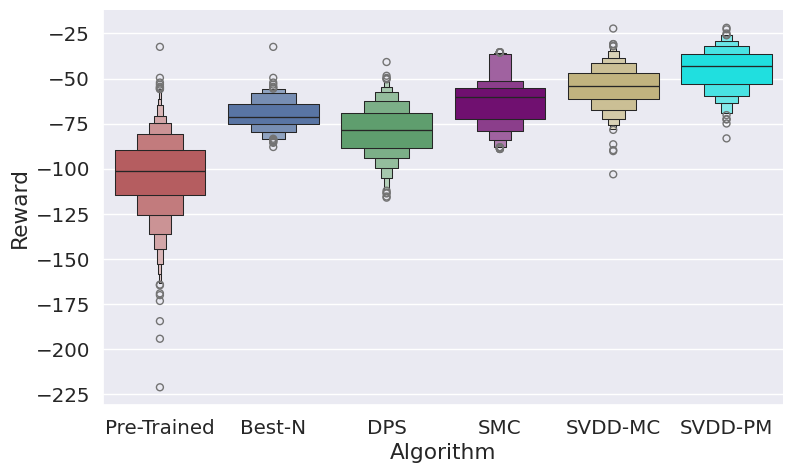
\includegraphics[width=.33\linewidth]{images/Images_compress.png}
    \label{fig:image_compress_distribution}}
    \subcaptionbox{Images: aesthetic score}{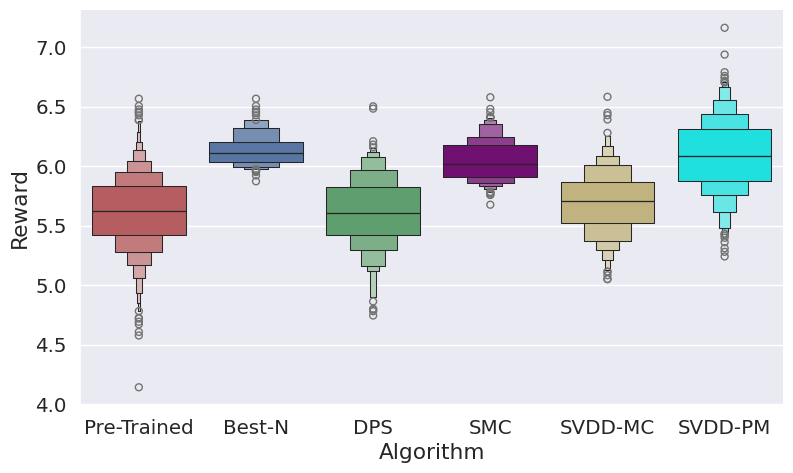
\includegraphics[width=.33\linewidth]{images/Images_asthetic.png}
    \label{fig:image2_asthetic_distribution}}  \\
    \subcaptionbox{Molecules: QED}{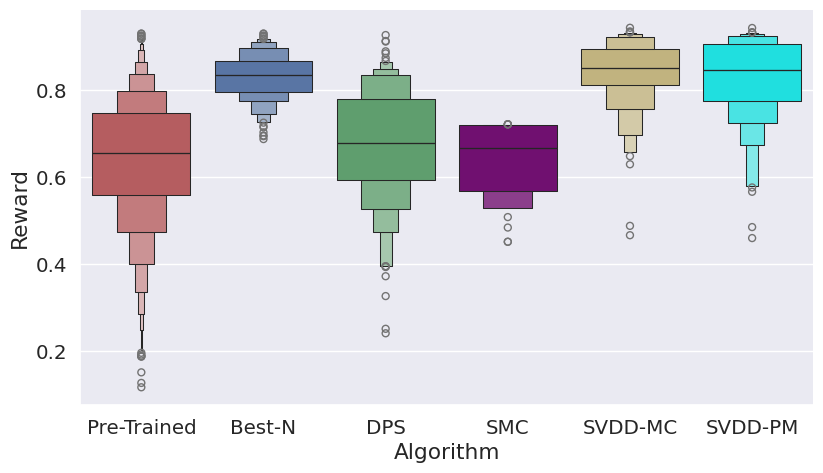
\includegraphics[width=.3\linewidth]{images/molecule_qed_distribution.png}
    \label{fig:molqed}} 
   \subcaptionbox{Molecules: SA}{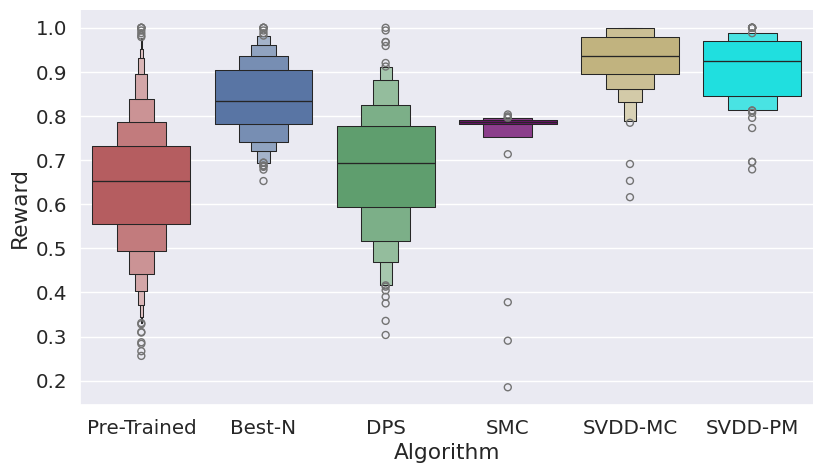
\includegraphics[width=.3\linewidth]{images/molecule_sa_distribution.png}
    \label{fig:molsa}}
    \subcaptionbox{Molecules: DS - parp1}{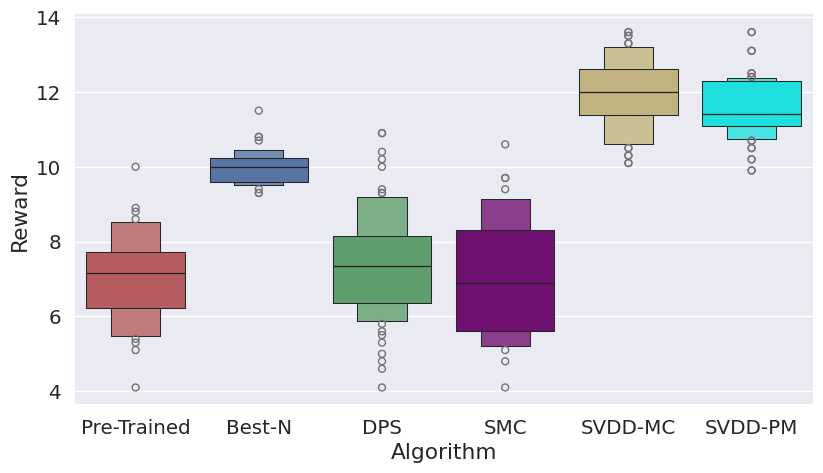
\includegraphics[width=.3\linewidth]{images/molecule_vina1_distribution.png}
    \label{fig:molecule_vina1}}
    \subcaptionbox{Molecules: DS - 5ht1b}{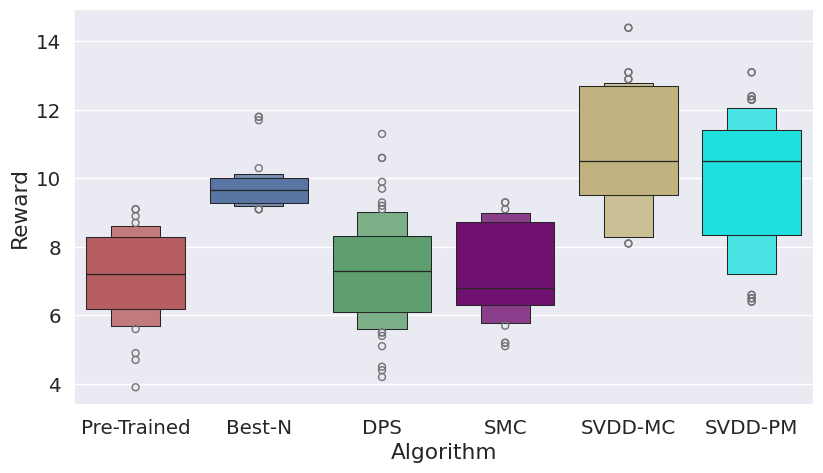
\includegraphics[width=.3\linewidth]{images/molecule_vina3_distribution.png}
    \label{fig:molecule_vina3}}
    \subcaptionbox{Molecules: DS - jak2}{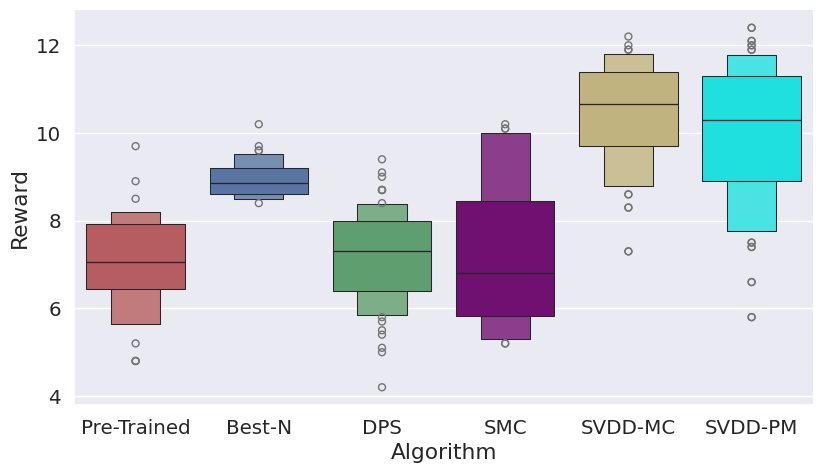
\includegraphics[width=.3\linewidth]{images/molecule_vina4_distribution.png}
    \label{fig:molecule_vina4}}
    \subcaptionbox{Molecules: DS - braf}{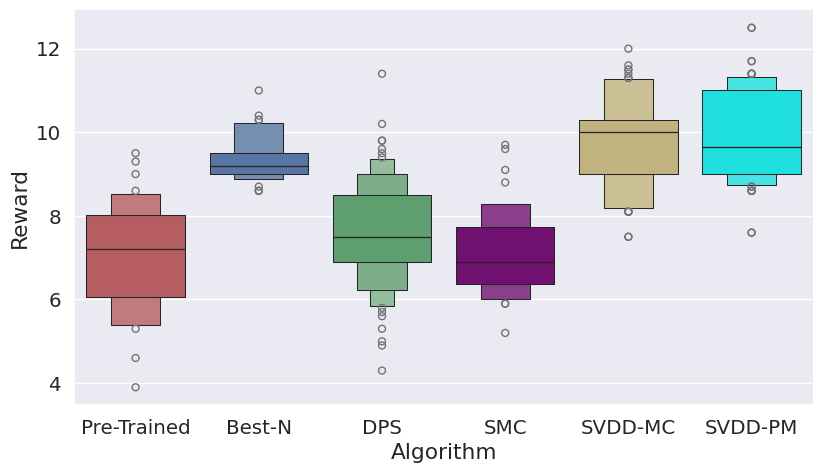
\includegraphics[width=.3\linewidth]{images/molecule_vina5_distribution.png}
    \label{fig:molecule_vina5}}
    \subcaptionbox{Enhancers}
{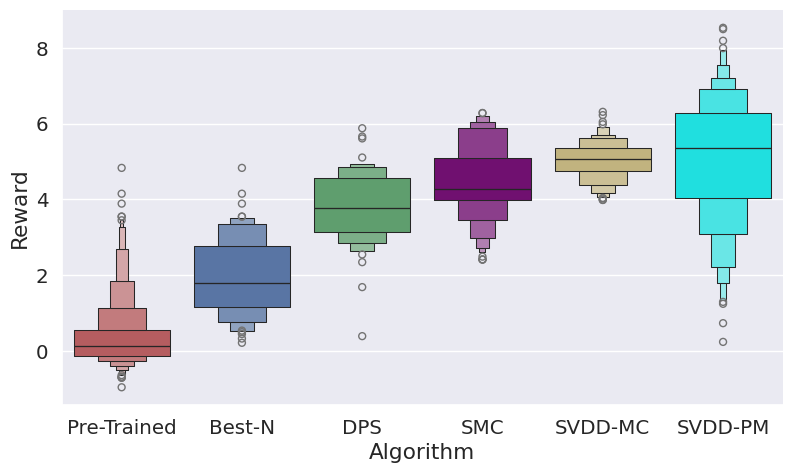
\includegraphics[width=.3\linewidth]{images/sequence_DNA.png}
    \label{fig:FNA}}
   \subcaptionbox{5'UTRs: MRL}{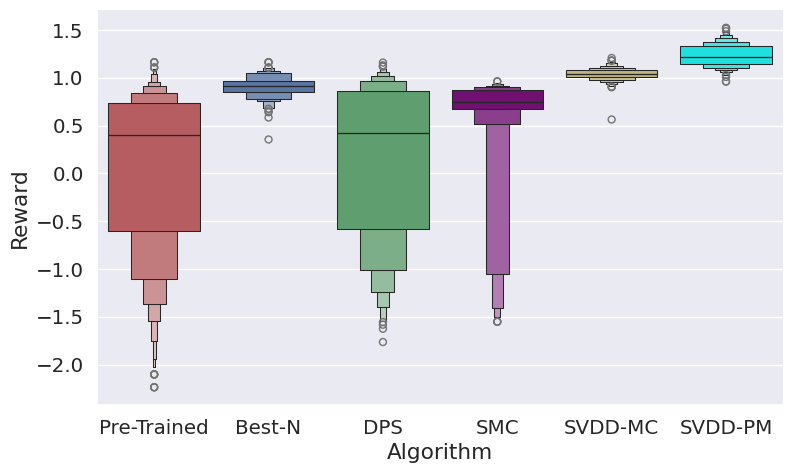
\includegraphics[width=.3\linewidth]{images/sequence_RNA.png}
    \label{fig:UTR_distribution}}
    \setlength{\belowcaptionskip}{-12pt}
\caption{We show the histogram of generated samples in terms of reward functions. We consistently observe that {\alg} demonstrates strong performances.   }

    \label{fig:proposal}
\end{figure}








\paragraph{Performance of value function training.} 

We report the performance of value function learning using Monte Carlo regression as follows in \alg-MC. In \pref{fig:training_curve}, we plot the Pearson correlation on the test dataset for the Enhancer and 5'UTR tasks, as well as the test MSE for the molecular task of parp1 docking score.



\begin{figure}[!ht]
    \centering
    \subcaptionbox{5'UTR MRL}{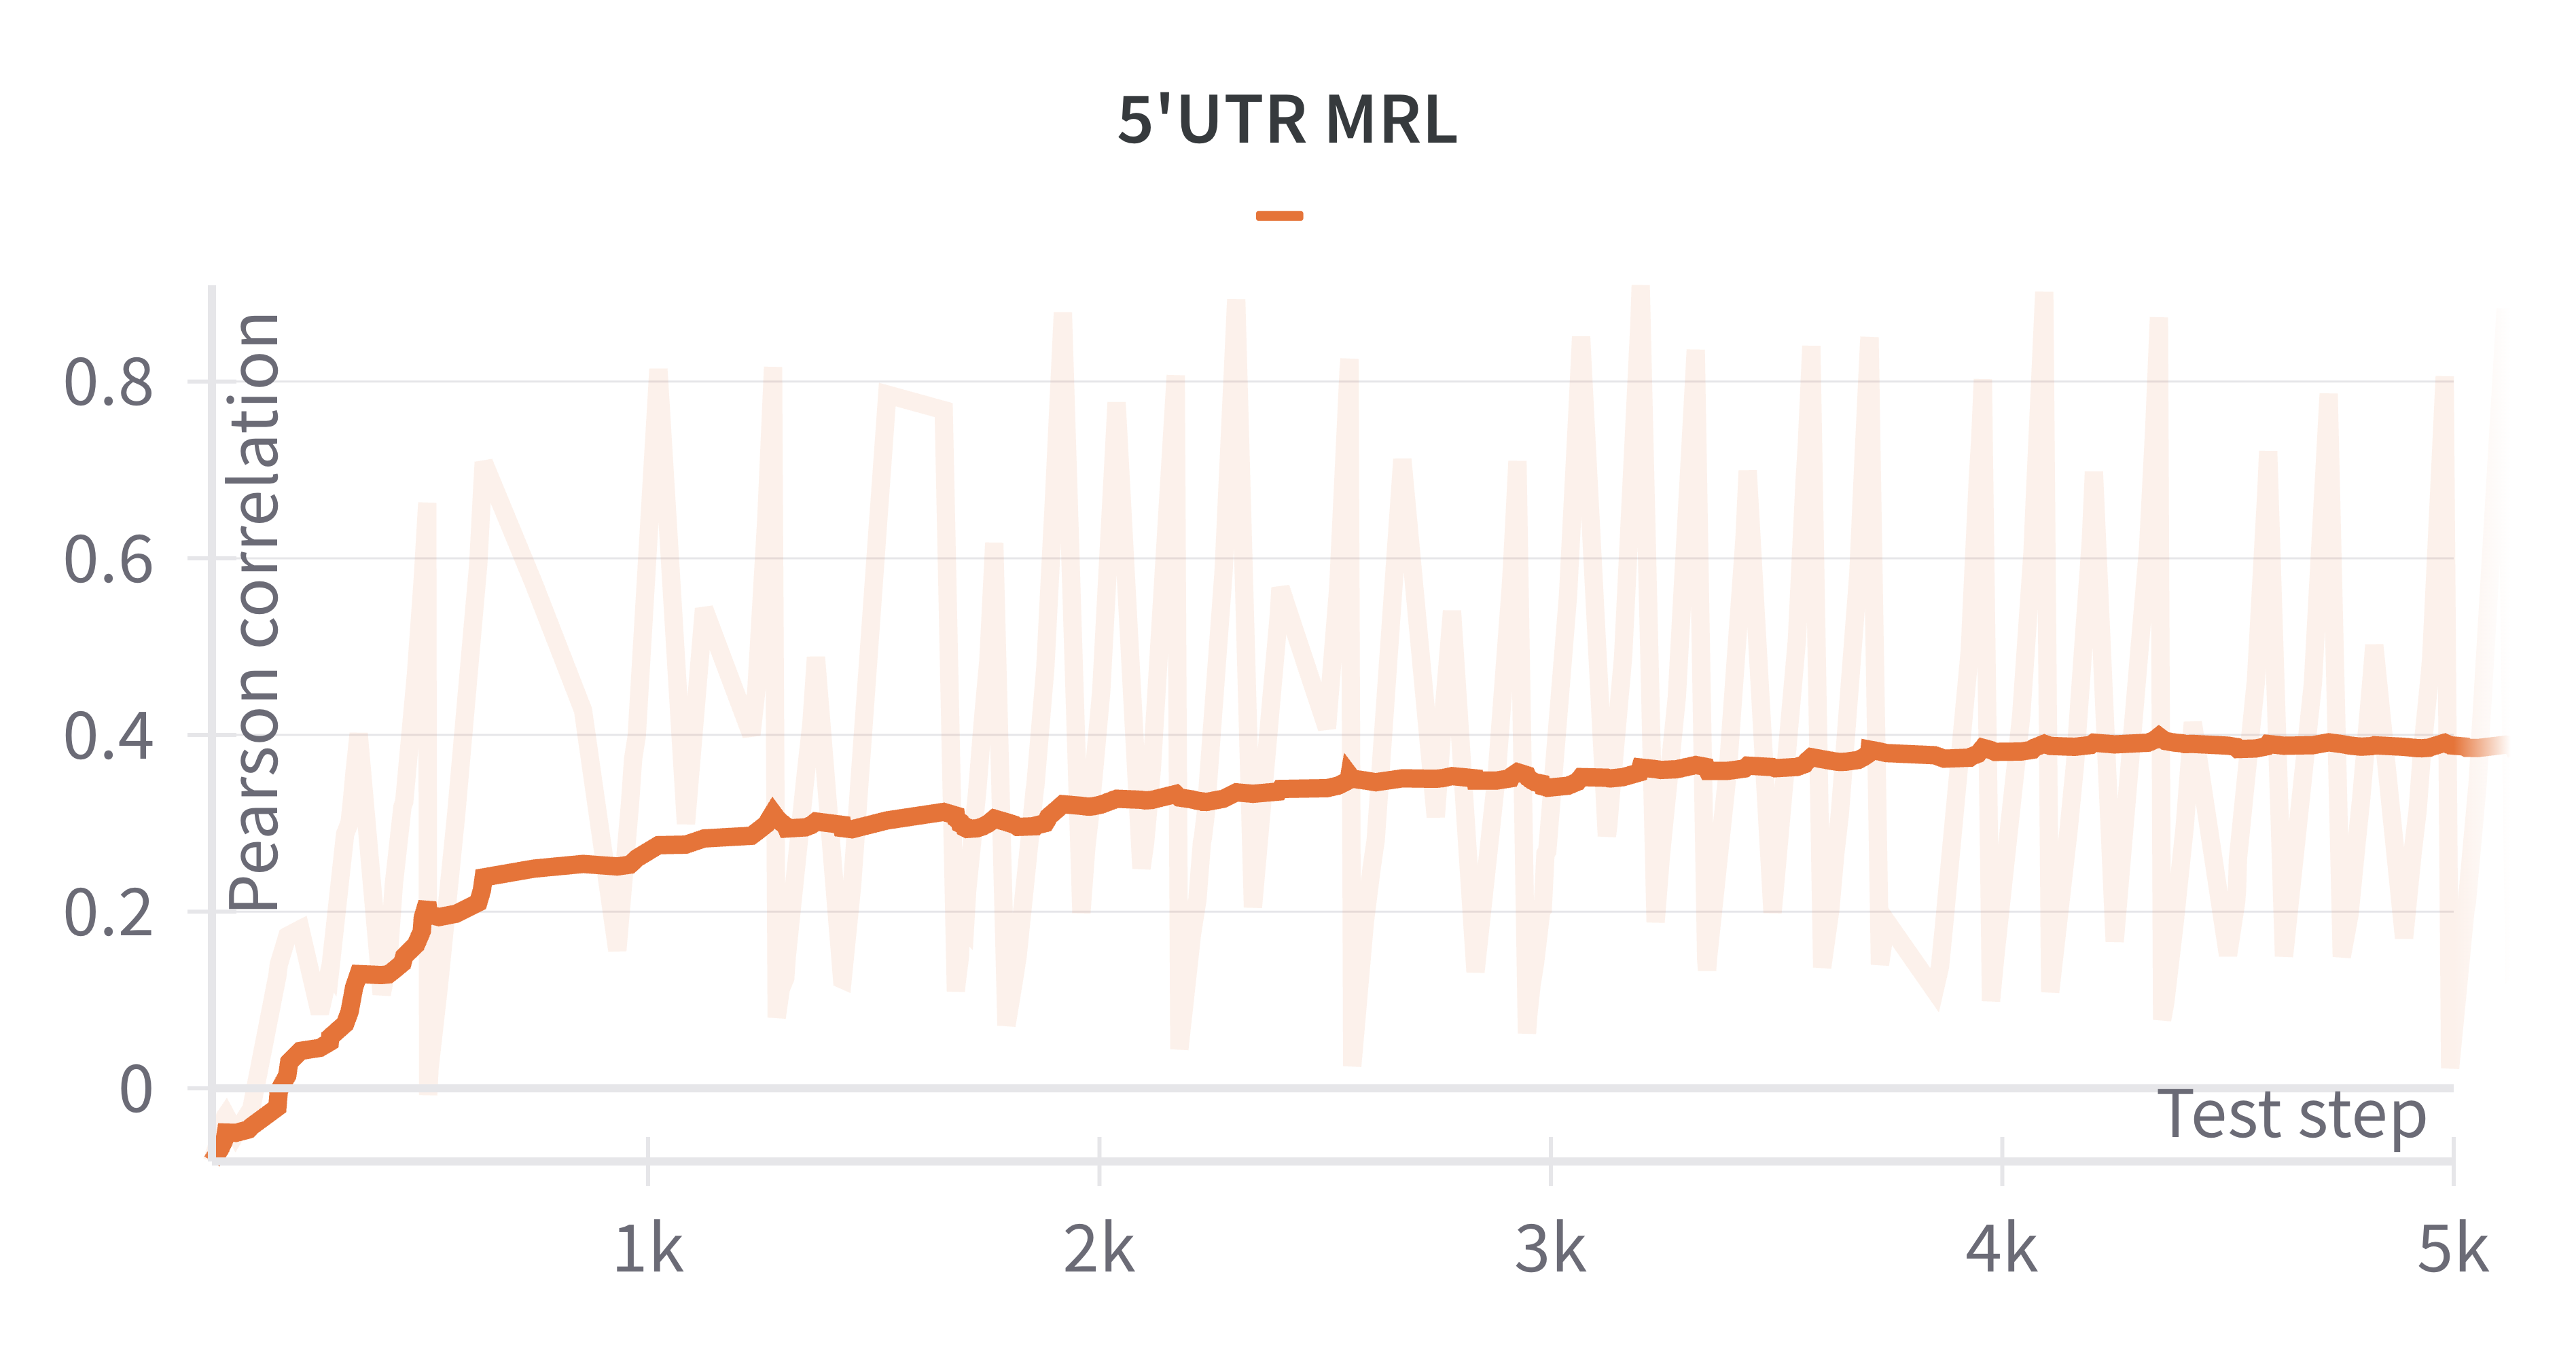
\includegraphics[width=.48\linewidth]{images/UTR_MRL.png}
    \label{fig:train_utr}}
    \subcaptionbox{Enhancers}{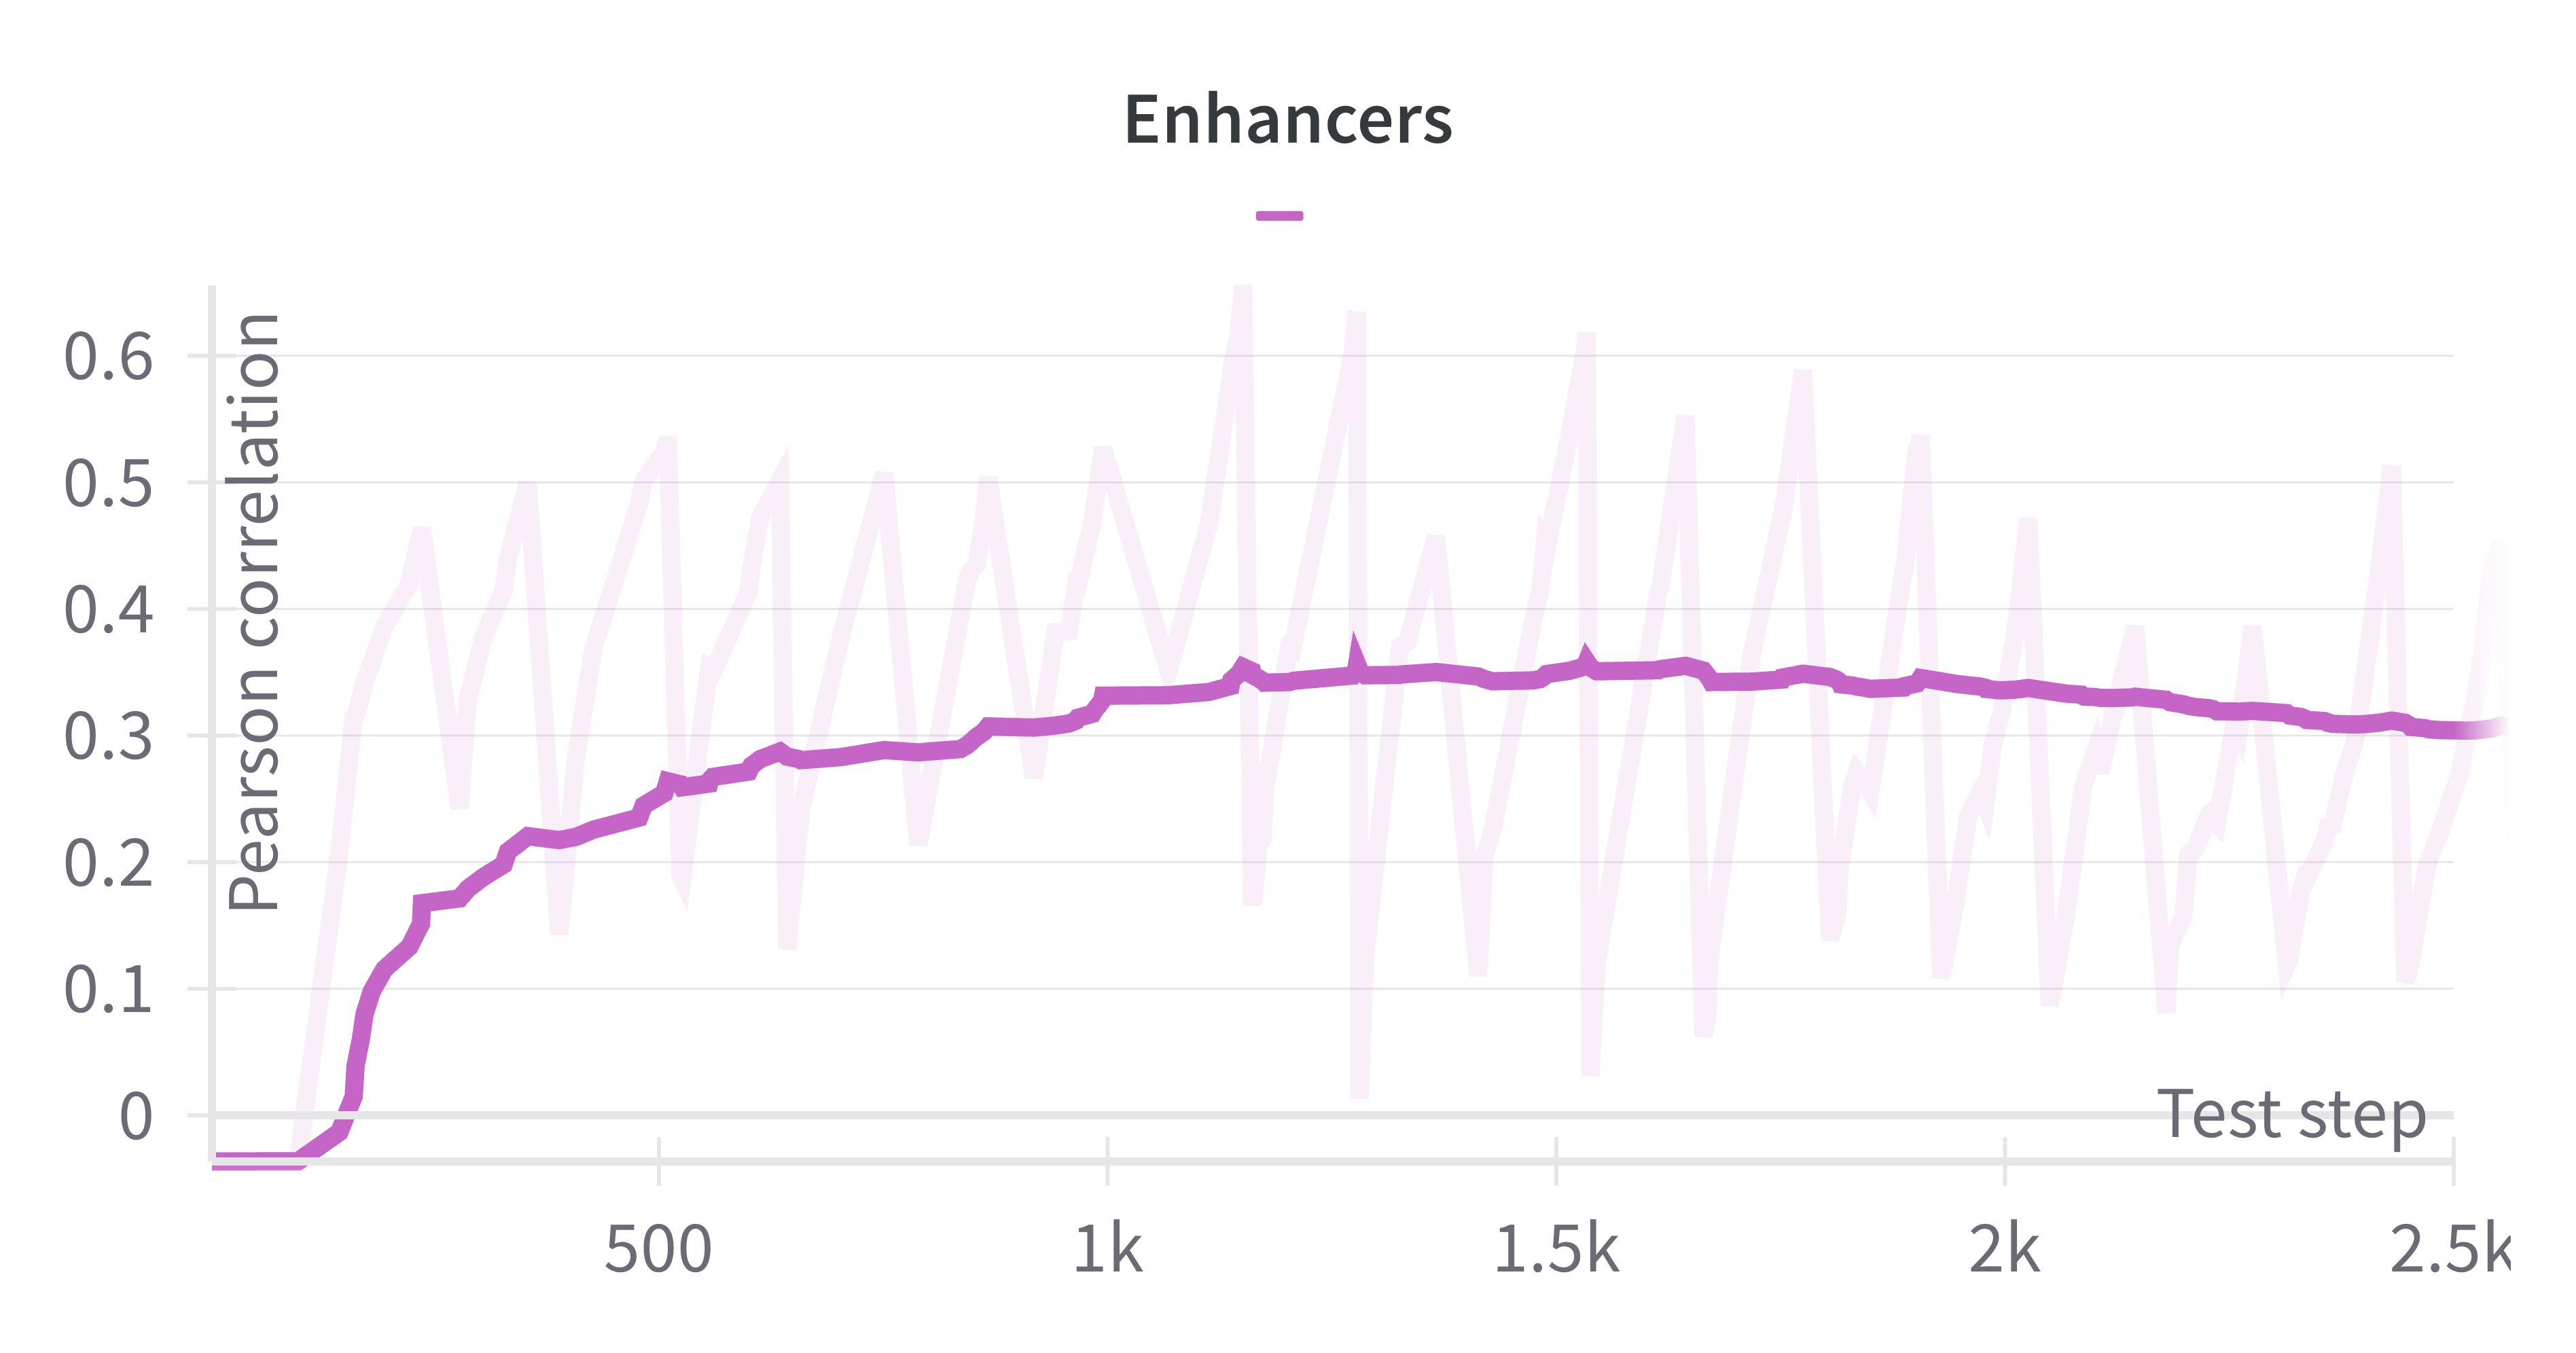
\includegraphics[width=.48\linewidth]{images/Enhancers.png}
    \label{fig:train_enhancer}} 
    \subcaptionbox{Molecules}{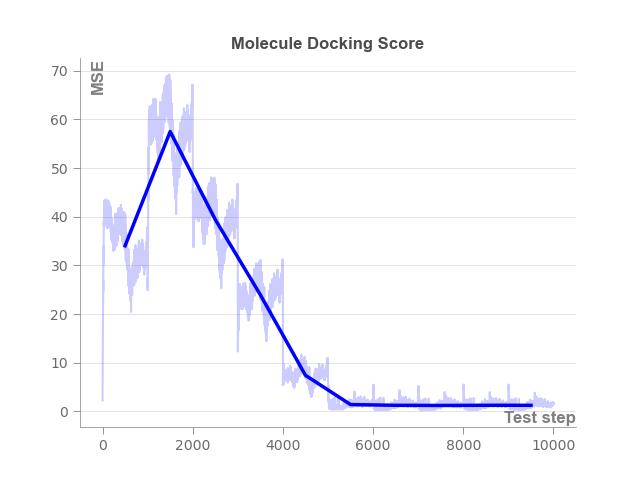
\includegraphics[width=.48\linewidth]{images/train_curve_vina1.png}
    \label{fig:train_mol_vina1}} 
    \caption{Training curve of value functions}
    \label{fig:training_curve}
\end{figure}


\paragraph{Validity metrics for molecule generation.} 



To evaluate the validity of our method in molecule generation, we report several key metrics that capture different aspects of molecule quality and diversity in \pref{tab:molecle_metrics}. 


\begin{table}[!ht]
\centering
\caption{Comparison of the generated molecules of pre-trained GDSS model and SVDD applied on various metrics.}
\resizebox{\textwidth}{!}{
\begin{tabular}{lcccccccccc}
\toprule
\textbf{Method}  & \textbf{Valid} & \textbf{Unique} & \textbf{Novelty} & \textbf{FCD} & \textbf{SNN} & \textbf{Frag/Test} & \textbf{Scaf} & \textbf{NSPDK MMD} & \textbf{Mol Stable} & \textbf{Atm Stable}\\
\midrule
Pre-trained  & \textbf{1.0} & \textbf{1.0} & \textbf{1.0} & 22.2799 & 0.2992 & \textbf{0.8274} & 0.0033 & \textbf{0.0260} & 0.2903 & \textbf{0.9256}\\
SVDD  & \textbf{1.0} & 0.9375 & \textbf{1.0} & \textbf{21.5671} & \textbf{0.3441} & 0.7803 & \textbf{0.0838} & 0.0772 & \textbf{0.4783} & 0.9095\\
\bottomrule
\end{tabular}
}
\label{tab:molecle_metrics}
\end{table}




The validity of a molecule indicates its adherence to chemical rules, defined by whether it can be successfully converted to SMILES strings by RDKit. Uniqueness refers to the proportion of generated molecules that are distinct by SMILES string. Novelty measures the percentage of the generated molecules that are not present in the training set. Fréchet ChemNet Distance (FCD) measures the similarity between the generated molecules and the test set. The Similarity to Nearest Neighbors (SNN) metric evaluates how similar the generated molecules are to their nearest neighbors in the test set. Fragment similarity measures the similarity of molecular fragments between generated molecules and the test set. Scaffold similarity assesses the resemblance of the molecular scaffolds in the generated set to those in the test set. The neighborhood subgraph pairwise distance kernel Maximum Mean Discrepancy (NSPDK MMD) quantifies the difference in the distribution of graph substructures between generated molecules and the test set considering node and edge features. Atom stability measures the percentage of atoms with correct bond valencies. Molecule stability measures the fraction of generated molecules that are chemically stable, \textit{i.e.}, whose all atoms have correct bond valencies. Specifically, atom and molecule stability are calculated using conformers generated by RDKit and optimized with UFF (Universal Force Field) and MMFF (Merck Molecular Force Field). 

We compare the metrics using 512 molecules generated from the pre-trained GDSS model and from SVDD optimizing SA, as shown in Table~\ref{tab:molecle_metrics}. Overall, our method achieves comparable performances with the pre-trained model on all metrics, maintaining high validity, novelty, and uniqueness while outperforming on several metrics such as molecule stability, FCD, SNN, and scaffold similarity. These results indicate that our approach can generate a diverse set of novel molecules that are chemically plausible and relevant.


\paragraph{More Ablation Studies.}

We provide several more ablation studies regarding $M$ on top of the results in the main text, as plotted in \pref{fig:additional_ablatation}. The results are consistent with what we have observed in \pref{fig:abletation}.

\begin{figure}[!ht]
\begin{subfigure}[c]{0.40\textwidth}
    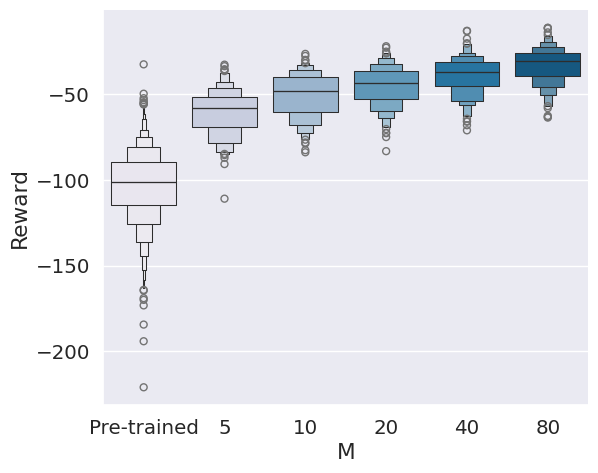
\includegraphics[width=\textwidth]{images/change_K_compress.png}
    \caption{Performance of {\alg} as $M$ varies. }
    \label{fig:change_k_compress}
\end{subfigure} 
    \begin{subfigure}[c]{0.6\textwidth}
    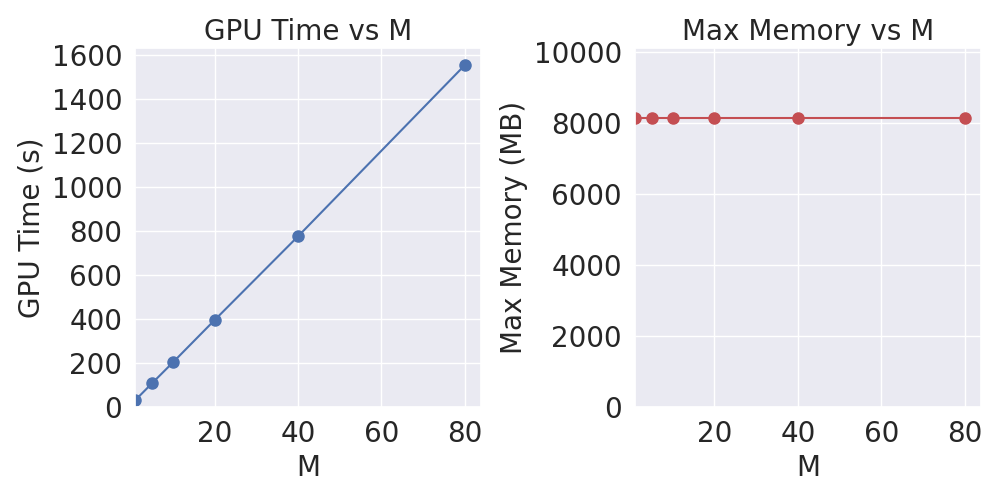
\includegraphics[width=\textwidth]{images/gpu_memory_time_plot_compress.png}
    \caption{GPU time and max memory of {\alg} as $M$ varies.}
    \label{fig:gpu_time_memory_compress}
\end{subfigure} 
\caption{Abltation Studies (for image generation while optimizing the compressibility) }
 \label{fig:additional_ablatation}
\end{figure}






\paragraph{Visualization of more generated samples.} 

We provide additional generated samples in this section. \pref{fig:images1} and \pref{fig:images2} show comparisons of generated images from baseline methods and {\alg} with different M values regarding compressibility and aesthetic score, respectively. \pref{fig:qed} and \pref{fig:sa} presents the comparisons of visualized molecules generated from the baseline model and {\alg} regarding QED and SA, respectively. The visualizations validate the strong performances of {\alg}. Given that {\alg} can achieve optimal SA for many molecules, we also visualize some molecules with optimal SA generated by {\alg}, as shown in \pref{fig:sa1.0}. In \pref{fig:vina1}, \pref{fig:vina3}, \pref{fig:vina4}, and \pref{fig:vina5} we visualizes the docking of \alg-generated molecular ligands to proteins parp1, 5ht1b, jak2, and braf, respectively. Docking scores presented above each column quantify the binding affinity of the ligand-protein interaction, while the figures include various representations and perspectives of the ligand-protein complexes.
We aim to provide a complete picture of how each ligand is situated within both the local binding environment and the larger structural framework of the protein.
First rows show close-up views of the ligand bound to the protein surface, displaying the topography and electrostatic properties of the protein's binding pocket and providing insight into the complementarity between the ligand and the pocket's surface. Second rows display distant views of the protein using the surface representation, offering a broader perspective on the ligand's spatial orientation within the global protein structure. Third rows provide close-up views of the ligand interaction using a ribbon diagram, which represents the protein's secondary structure, such as alpha-helices and beta-sheets, to highlight the specific regions of the protein involved in binding. Fourth rows show distant views of the entire protein structure in ribbon diagram, with ligands displayed within the context of the protein’s full tertiary structure.
Ligands generally fit snugly within the protein pocket, as evidenced by the close-up views in both the surface and ribbon diagrams, which show minimal steric clashes and strong surface complementarity. 


\begin{figure}[!th]
    \centering
    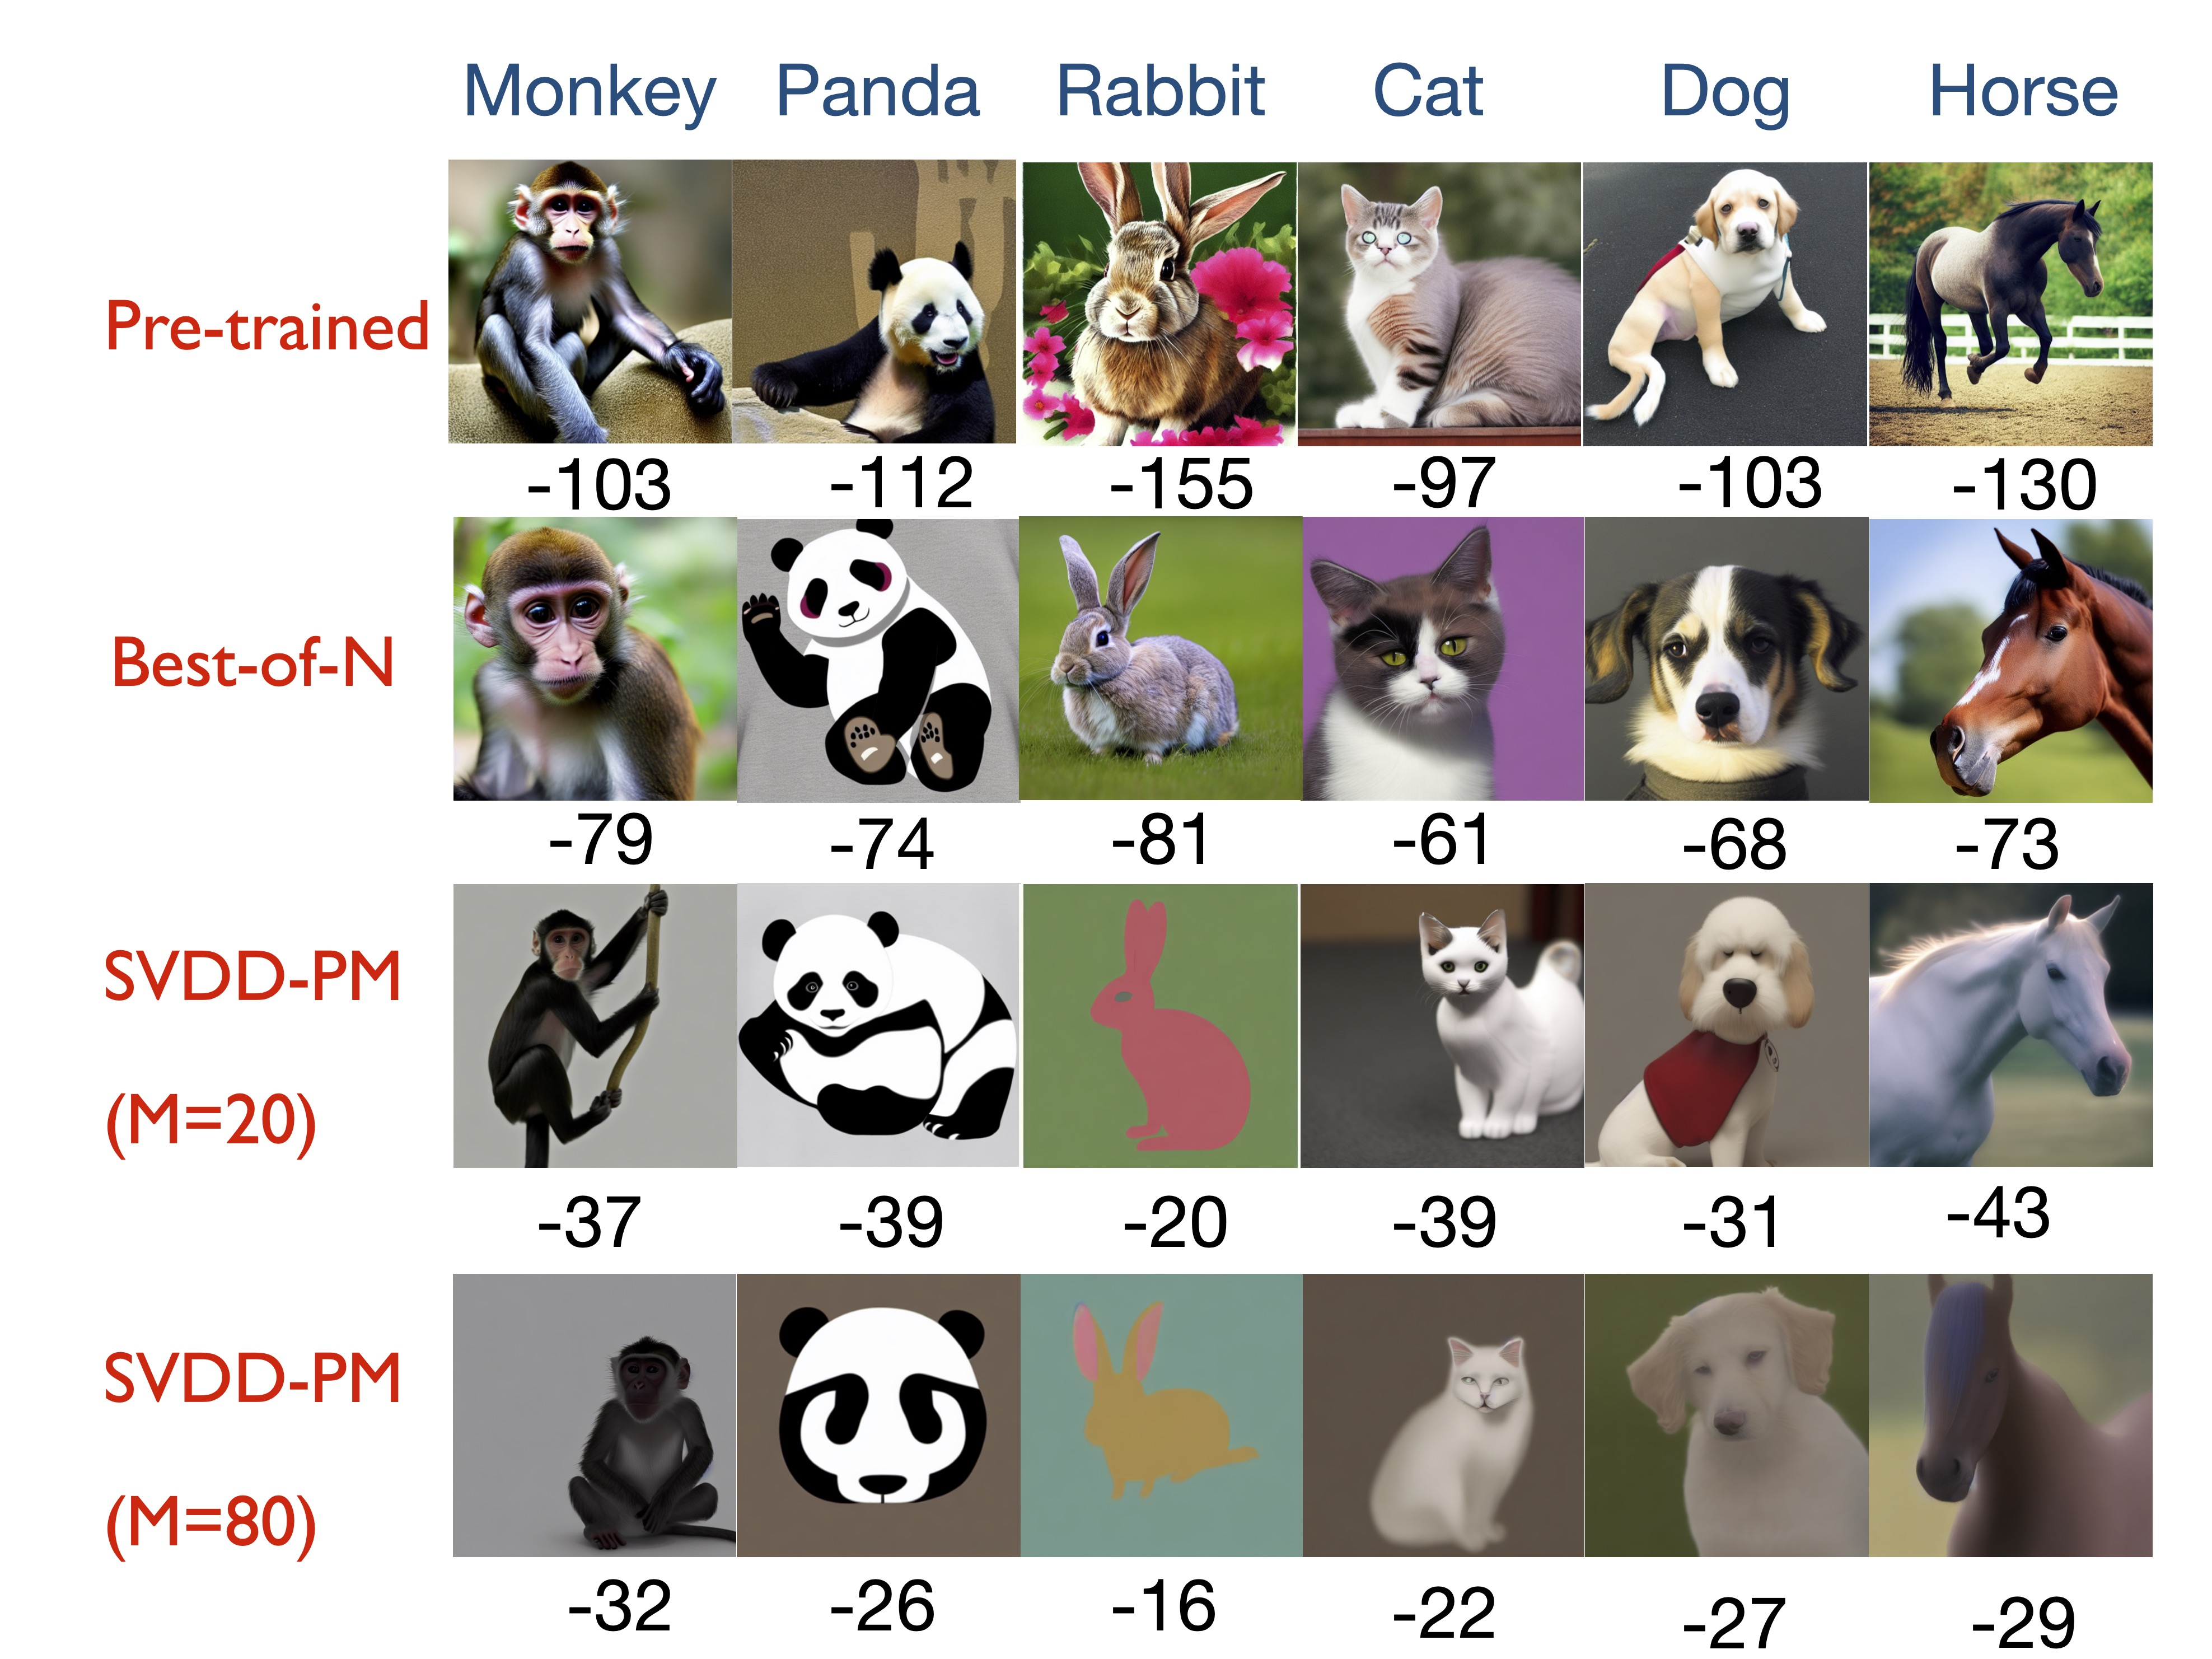
\includegraphics[width=1.0\linewidth]{images/Images_comp.jpg}  %
    \caption{Additional generated samples (Domain: images, Reward: Compressibility)}
    \label{fig:images1}
\end{figure}

\begin{figure}[!th]
    \centering
    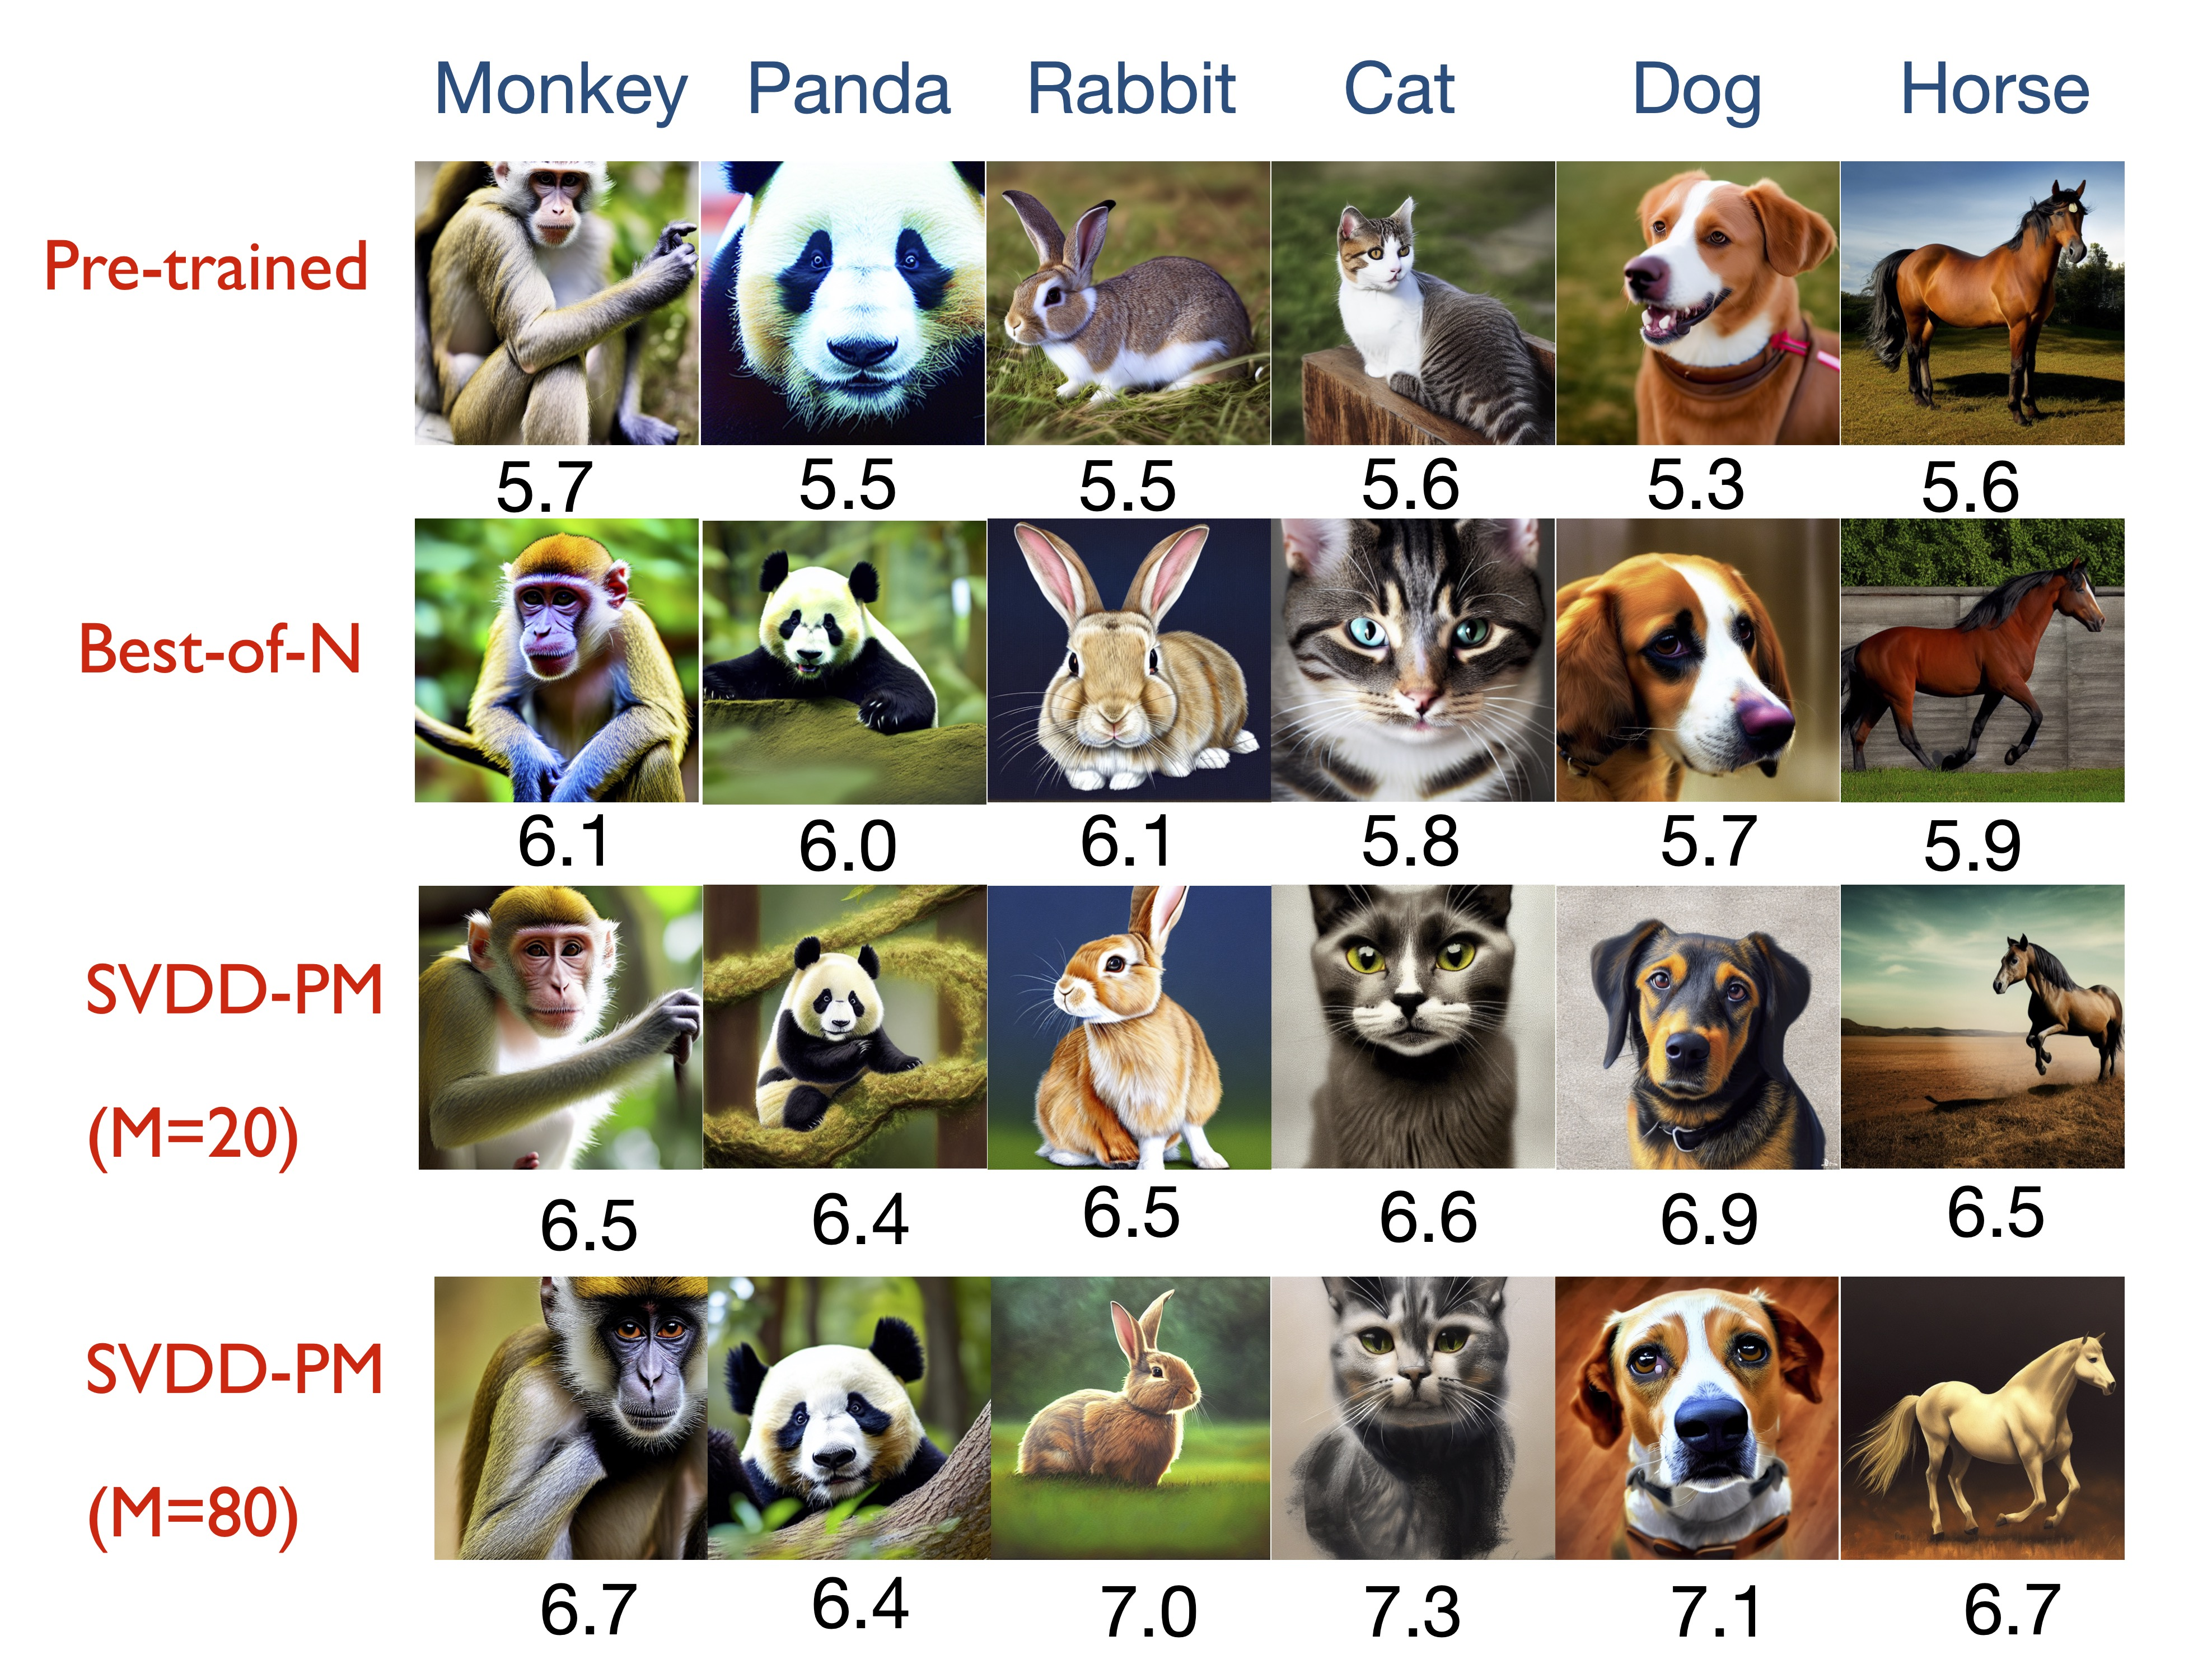
\includegraphics[width=1.0\linewidth]{images/Images_asthetic.jpg}  %
    \caption{Additional generated samples (Domain: Images, Reward: Aesthetic score)}
    \label{fig:images2}
\end{figure}

\begin{figure}[!th]
    \centering
    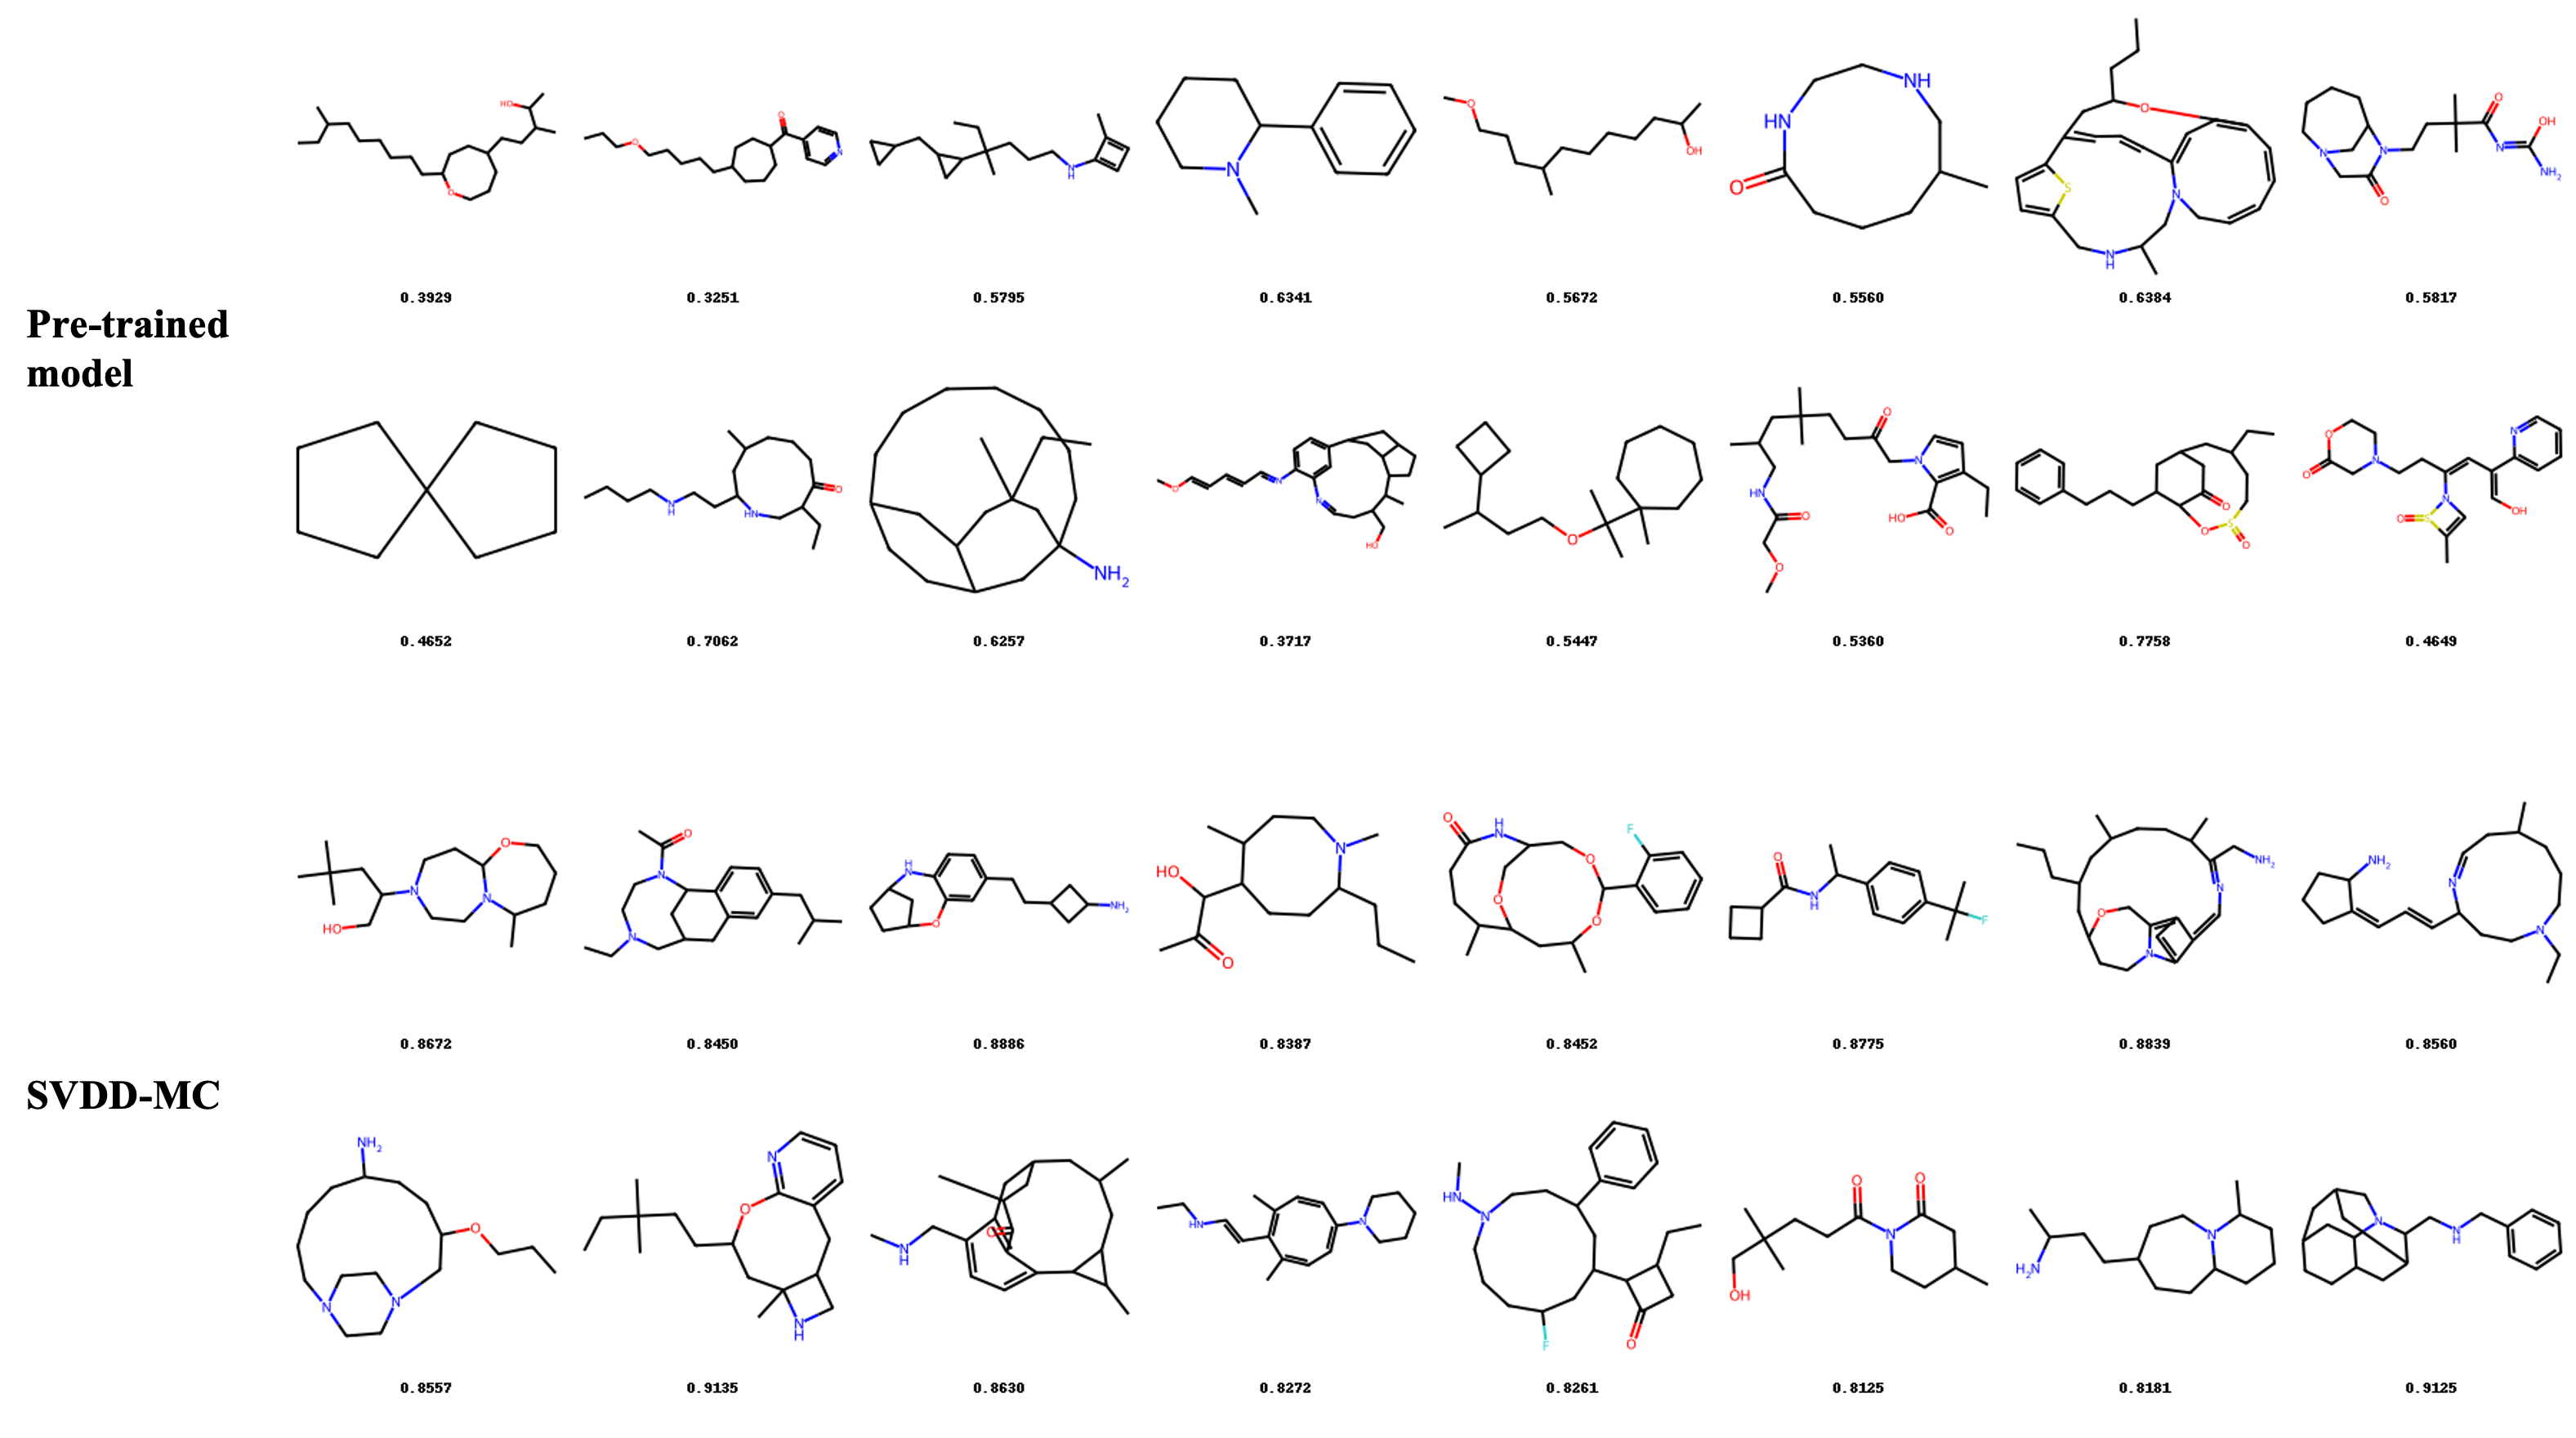
\includegraphics[width=1.0\linewidth]{images/qed.png}
    \caption{Additional generated samples (Domain: Molecules, Reward: QED score)}
    \label{fig:qed}
\end{figure}

\begin{figure}[!th]
    \centering
    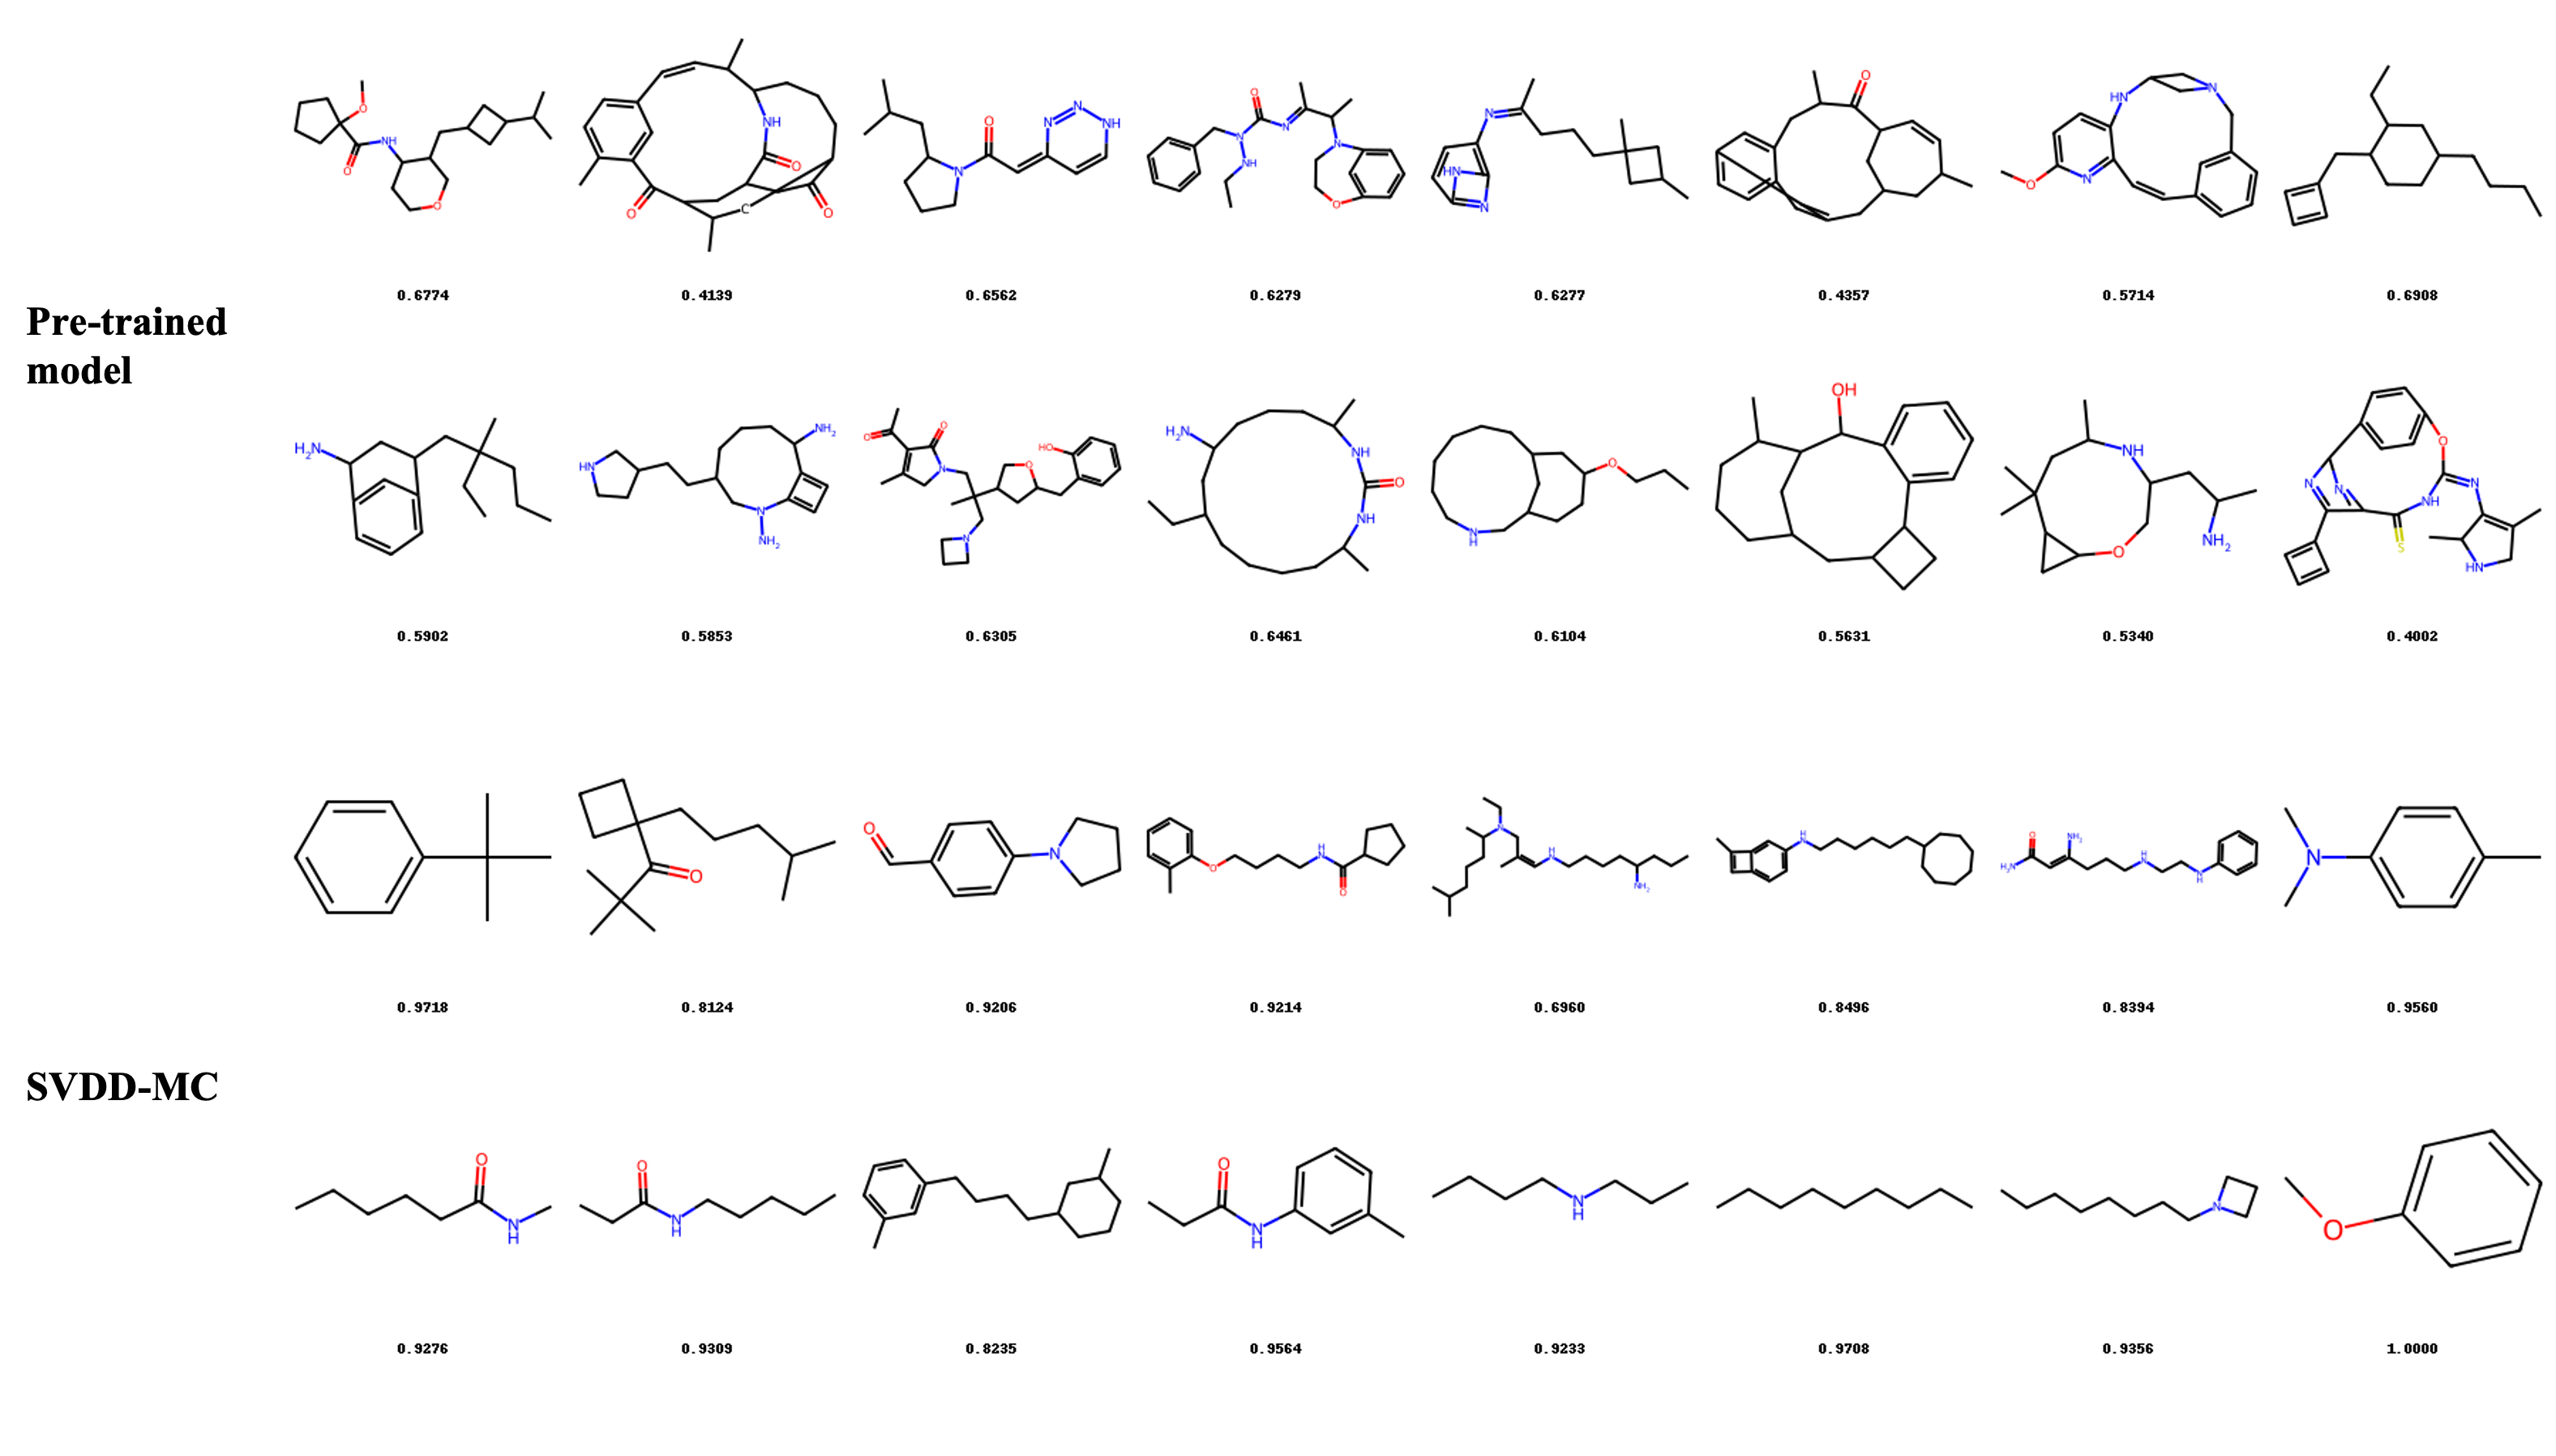
\includegraphics[width=1.0\linewidth]{images/sa.png}
    \caption{Additional generated samples (Domain: Molecules, Reward: SA score, normalized as $(10-SA)/9$)}
    \label{fig:sa}
\end{figure}

\begin{figure}[!th]
    \centering
    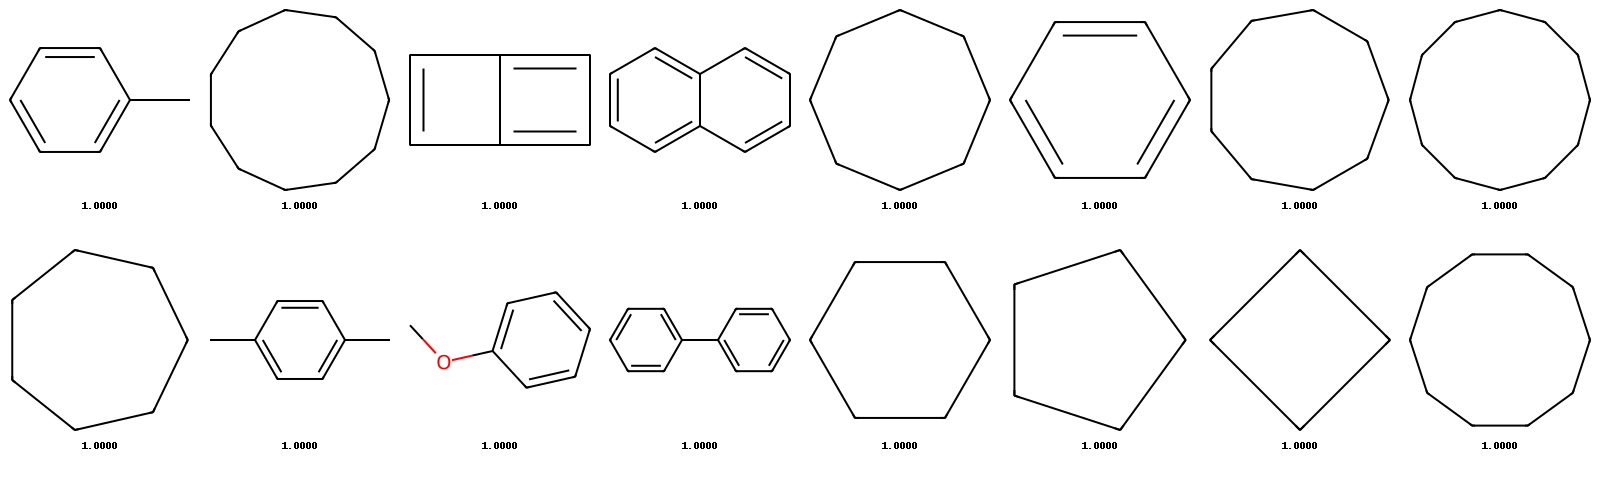
\includegraphics[width=1.0\linewidth]{images/molecule_SA1.0_grid_zinc_ours.png}
    \caption{Additional generated samples from {\alg}-MC (Domain: Molecules, Reward: SA score = 1.0 (normalized as $(10-SA)/9$))}
    \label{fig:sa1.0}
\end{figure}

\begin{figure}[!th]
    \centering
    \includegraphics[width=1.0\linewidth]{images/mol_vina_plot_pymol_grid.png}
    \caption{Additional generated samples from {\alg} (Domain: Molecules, Reward: Docking score - parp1 (normalized as $max(-DS, 0)$)) }
    \label{fig:vina1}
\end{figure}

\begin{figure}[!th]
    \centering
    \includegraphics[width=1.0\linewidth]{images/mol_vina3_plot_pymol_grid.png}
    \caption{Additional generated samples from {\alg} (Domain: Molecules, Reward: Docking score - 5ht1b (normalized as $max(-DS, 0)$))}
    \label{fig:vina3}
\end{figure}

\begin{figure}[!th]
    \centering
    \includegraphics[width=1.0\linewidth]{images/mol_vina4_plot_pymol_grid.png}
    \caption{Additional generated samples from {\alg} (Domain: Molecules, Reward: Docking score - jak2 (normalized as $max(-DS, 0)$))}
    \label{fig:vina4}
\end{figure}

\begin{figure}[!th]
    \centering
    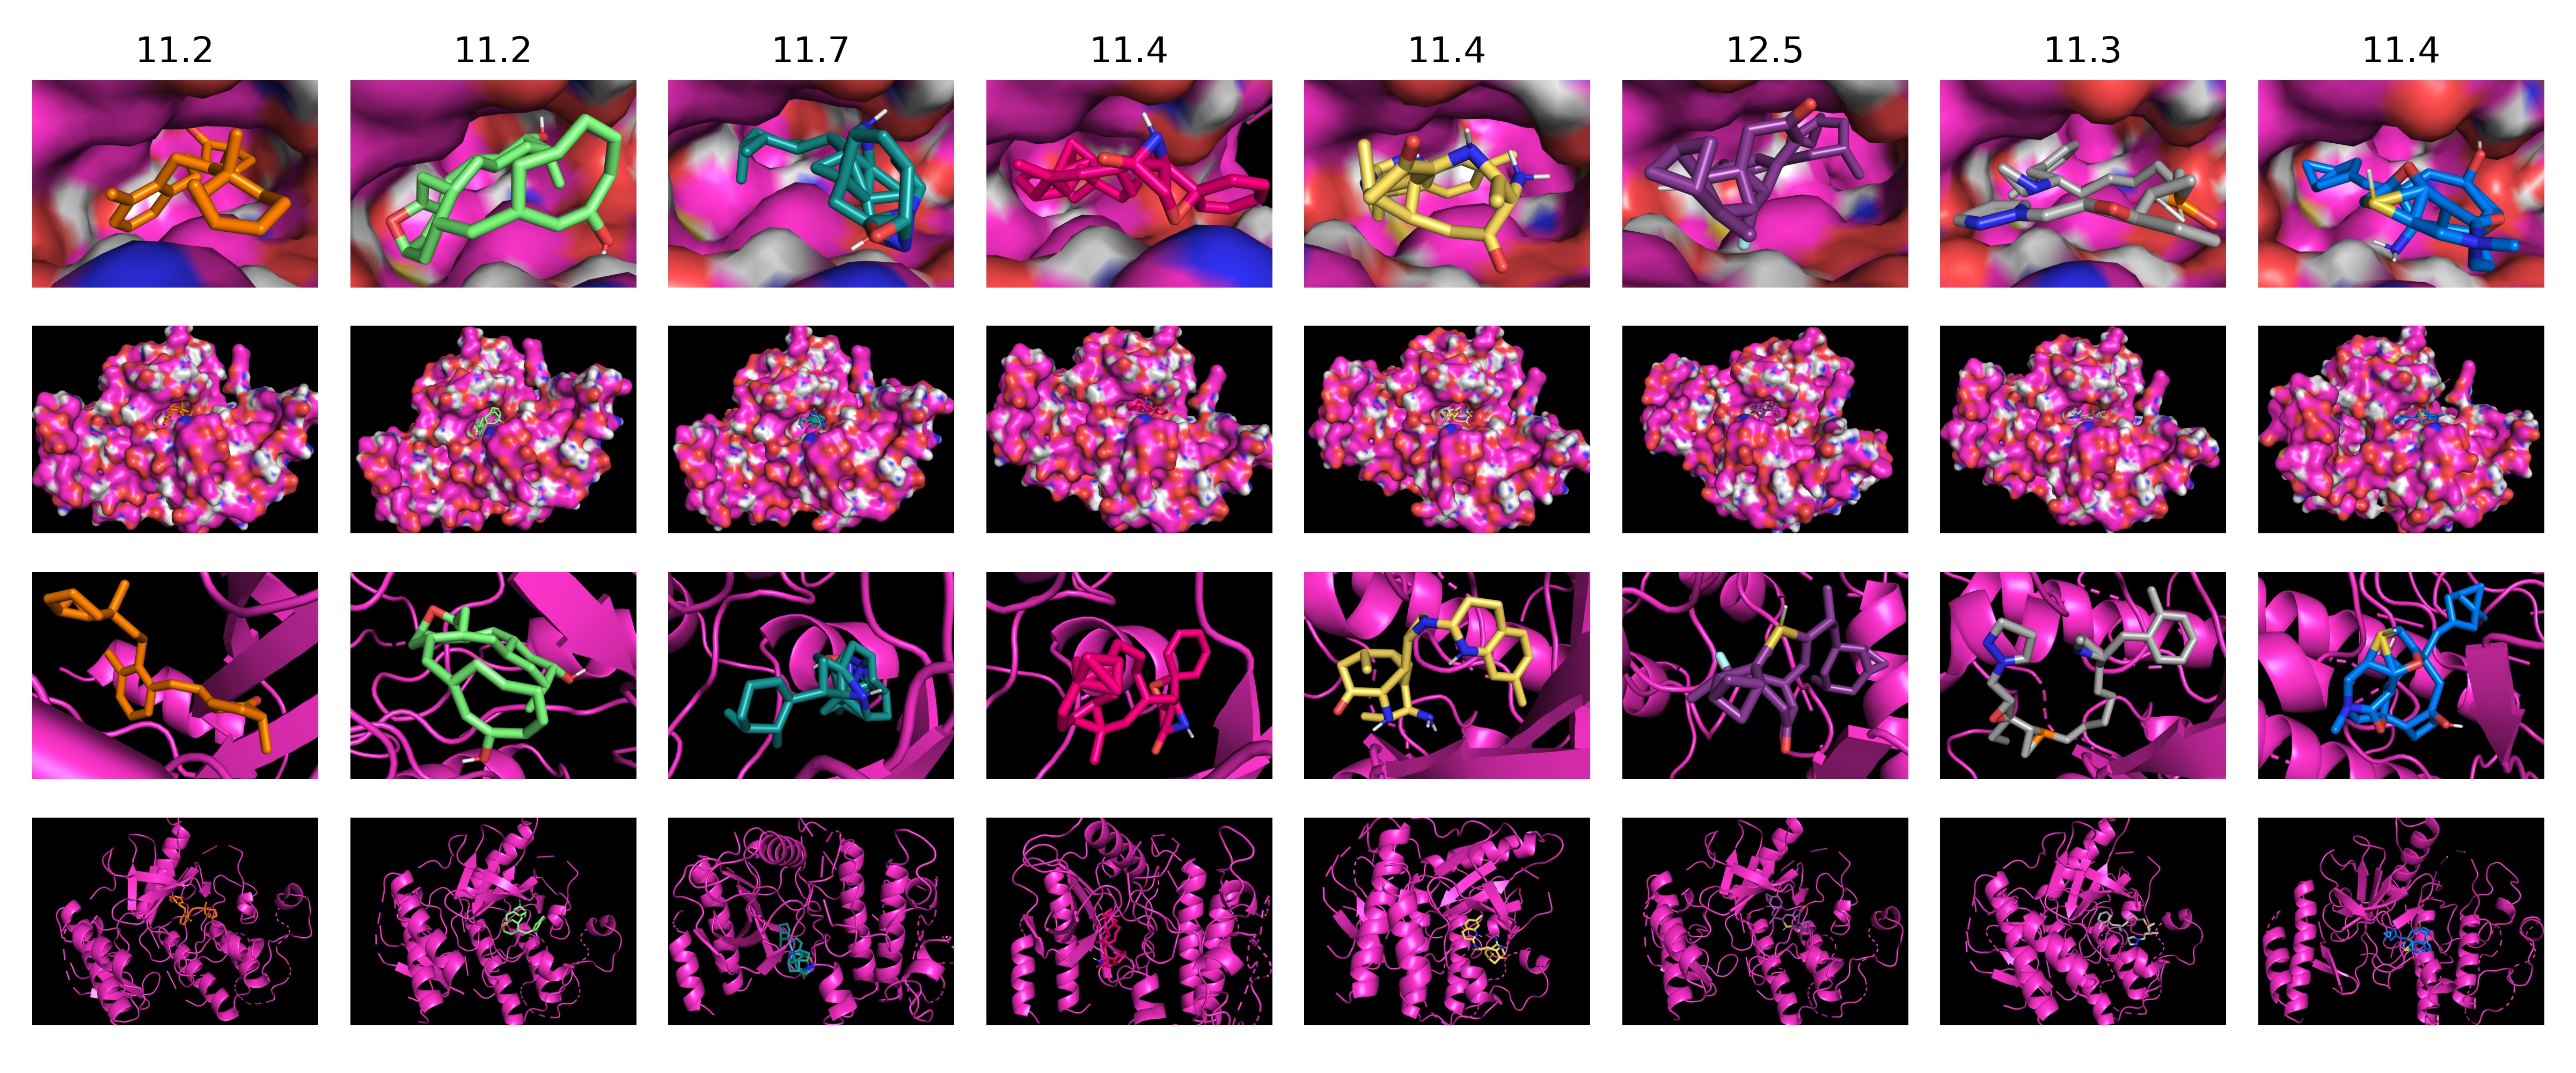
\includegraphics[width=1.0\linewidth]{images/mol_vina5_plot_pymol_grid.jpg} %
    \caption{Additional generated samples from {\alg} (Domain: Molecules, Reward: Docking score - braf (normalized as $max(-DS, 0)$))}
    \label{fig:vina5}
\end{figure}